\documentclass[hyperref=colorlinks]{beamer}
\mode<presentation>
\usetheme{iclpt}
\setbeamertemplate{navigation symbols}{}
\setbeamertemplate{headline}{
\begin{beamercolorbox}[leftskip=.2cm,rightskip=.2cm,topskip=.2cm,ht=1.1cm,dp=0.1cm,wd=\textwidth]{institute in head/foot}
  
\includegraphics[height=1cm]{icl.pdf}
  \hfill
  
\includegraphics[height=1cm]{../Pics/CMS-Color.pdf}
\end{beamercolorbox}
}
\setbeamertemplate{footline}{
\begin{beamercolorbox}[ht=.55cm,dp=0.4cm,wd=\textwidth,leftskip=.3cm]{author in head/foot}%
  \begin{minipage}[c]{5cm}%
    \usebeamerfont{author in head/foot}
    \insertshortauthor 
    \insertshorttitle
    \end{minipage}\hfill%
  \insertframenumber{} / \pageref{lastframe}
  \hfill
  \begin{minipage}{6cm}
    \hfill
  \end{minipage}
\end{beamercolorbox}%
}

\usepackage{color}
\usepackage{tabularx,colortbl}
\usepackage{graphicx}
\usepackage{pdfpages}
\usepackage{feynmp}
\DeclareGraphicsRule{*}{mps}{*}{}

\title{\vspace{-0.2cm} Trigger Efficiency Measurements in Re-Reco Data}
%\subtitle{Paper - HIG-13-030, PASs: HIG-13-013, HIG-13-018, HIG-13-028 \vspace{-0.7cm}}
\author[P. Dunne]{\underline{P. Dunne} }%\\ on behalf of the H$\rightarrow$invisible analysis groups} % A.M. Magnan and A. Nikitenko Joao Pela with \\ R. Aggleton, J. Brooke: Bristol \\ C.Asawangtrakuldee, Q.Li: Peking \\ P. Srimanobhas: Chulalongkorn \\ S. Kumar, K. Mazumdar: Mumbai}
\titlegraphic{
  \vspace{-0.7cm}
  %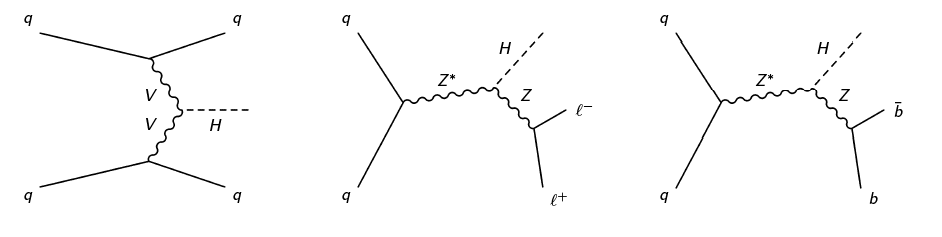
\includegraphics[width=\textwidth]{TalkPics/invcomb021213/feyndiags}
%% \begin{fmfgraph*}(100,70)
%%         \fmfleft{i1,i2}
%%         \fmfright{o1,o2,o3}
%%         \fmf{fermion}{i1,v1,o1}
%%         \fmf{fermion}{i2,v2,o3}
%%         \fmf{phantom,tension=4/5}{v1,v2}
%%         \fmffreeze
%%         \fmf{photon,label=$W,,Z$}{v1,v3}
%%         \fmf{photon,label=$W,,Z$}{v2,v3}
%%         \fmf{dashes}{v3,o2}
%%         \fmflabel{$q$}{i1}
%%         \fmflabel{$q$}{i2}
%%         \fmflabel{$q$}{o1}
%%         \fmflabel{$q$}{o3}
%%         \fmflabel{$H$}{o2}
%%       \end{fmfgraph*}
}
\date{}
\begin{document}
\begin{fmffile}{hig1330approvalfeynmandiags}

%TITLE PAGE
\section{Title}
\begin{frame}
  \titlepage
  
\end{frame}

%OUTLINE
\begin{frame}
  \frametitle{Overview}
  \begin{block}{}
    \scriptsize
  \begin{itemize}
  \item I have used the SingleMu primary dataset to measure the efficiency of our prompt and parked triggers
  \item[-] So far I only have the 1D efficiencies for each variable
  \item I have also measured the efficiency in each run separately
    \end{itemize}
  \end{block}
\end{frame}

\begin{frame}
  \frametitle{MET - Run by Run}
  \begin{block}{}
    \scriptsize
    \begin{itemize}
    \item All cuts except $\Delta\phi_{jj}$ and CJV have been applied
    \end{itemize}
  \end{block}
  \begin{columns}
    \column{.5\textwidth}
    \begin{block}{\scriptsize Run A}
      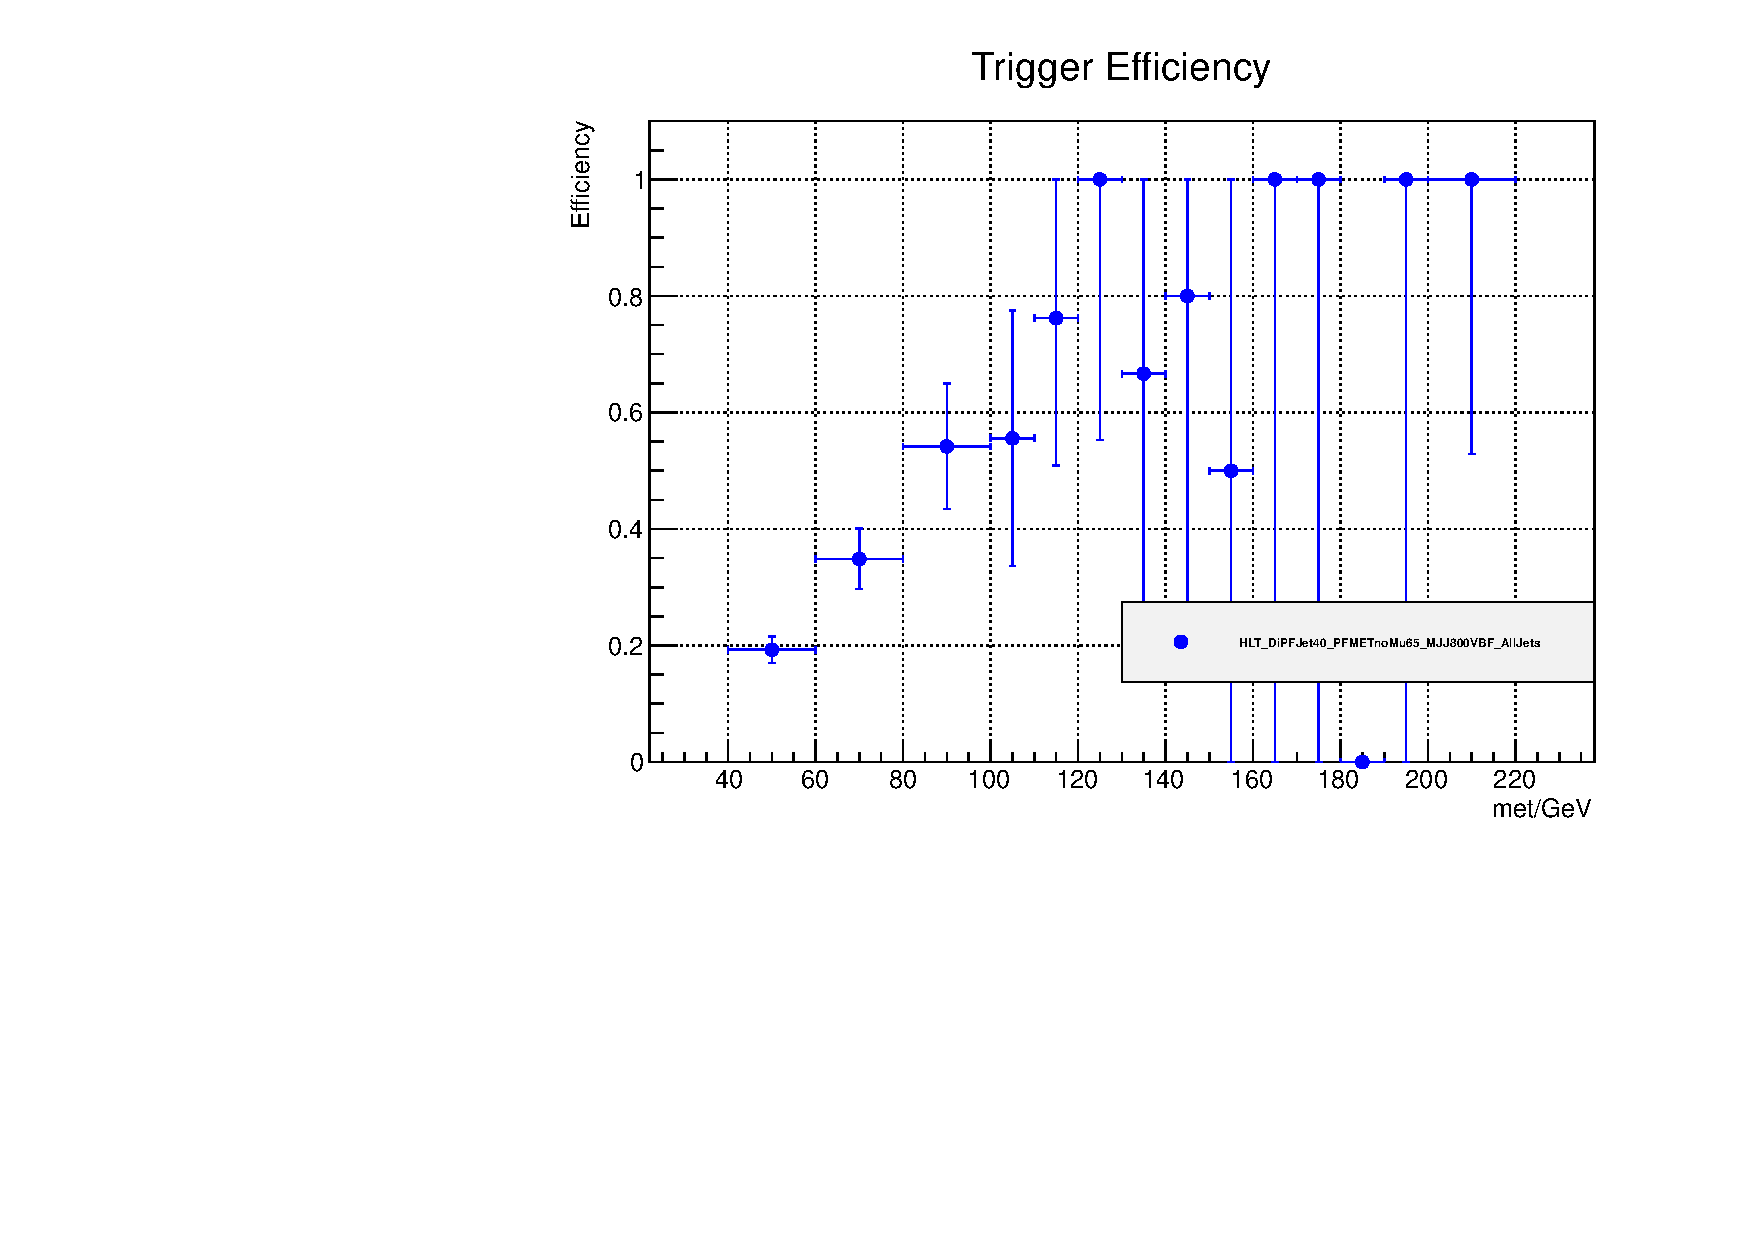
\includegraphics[width=\textwidth]{TalkPics/trigeffplots/metefficiency0.pdf}
    \end{block}
    \column{.5\textwidth}
    \begin{block}{\scriptsize Run B}
      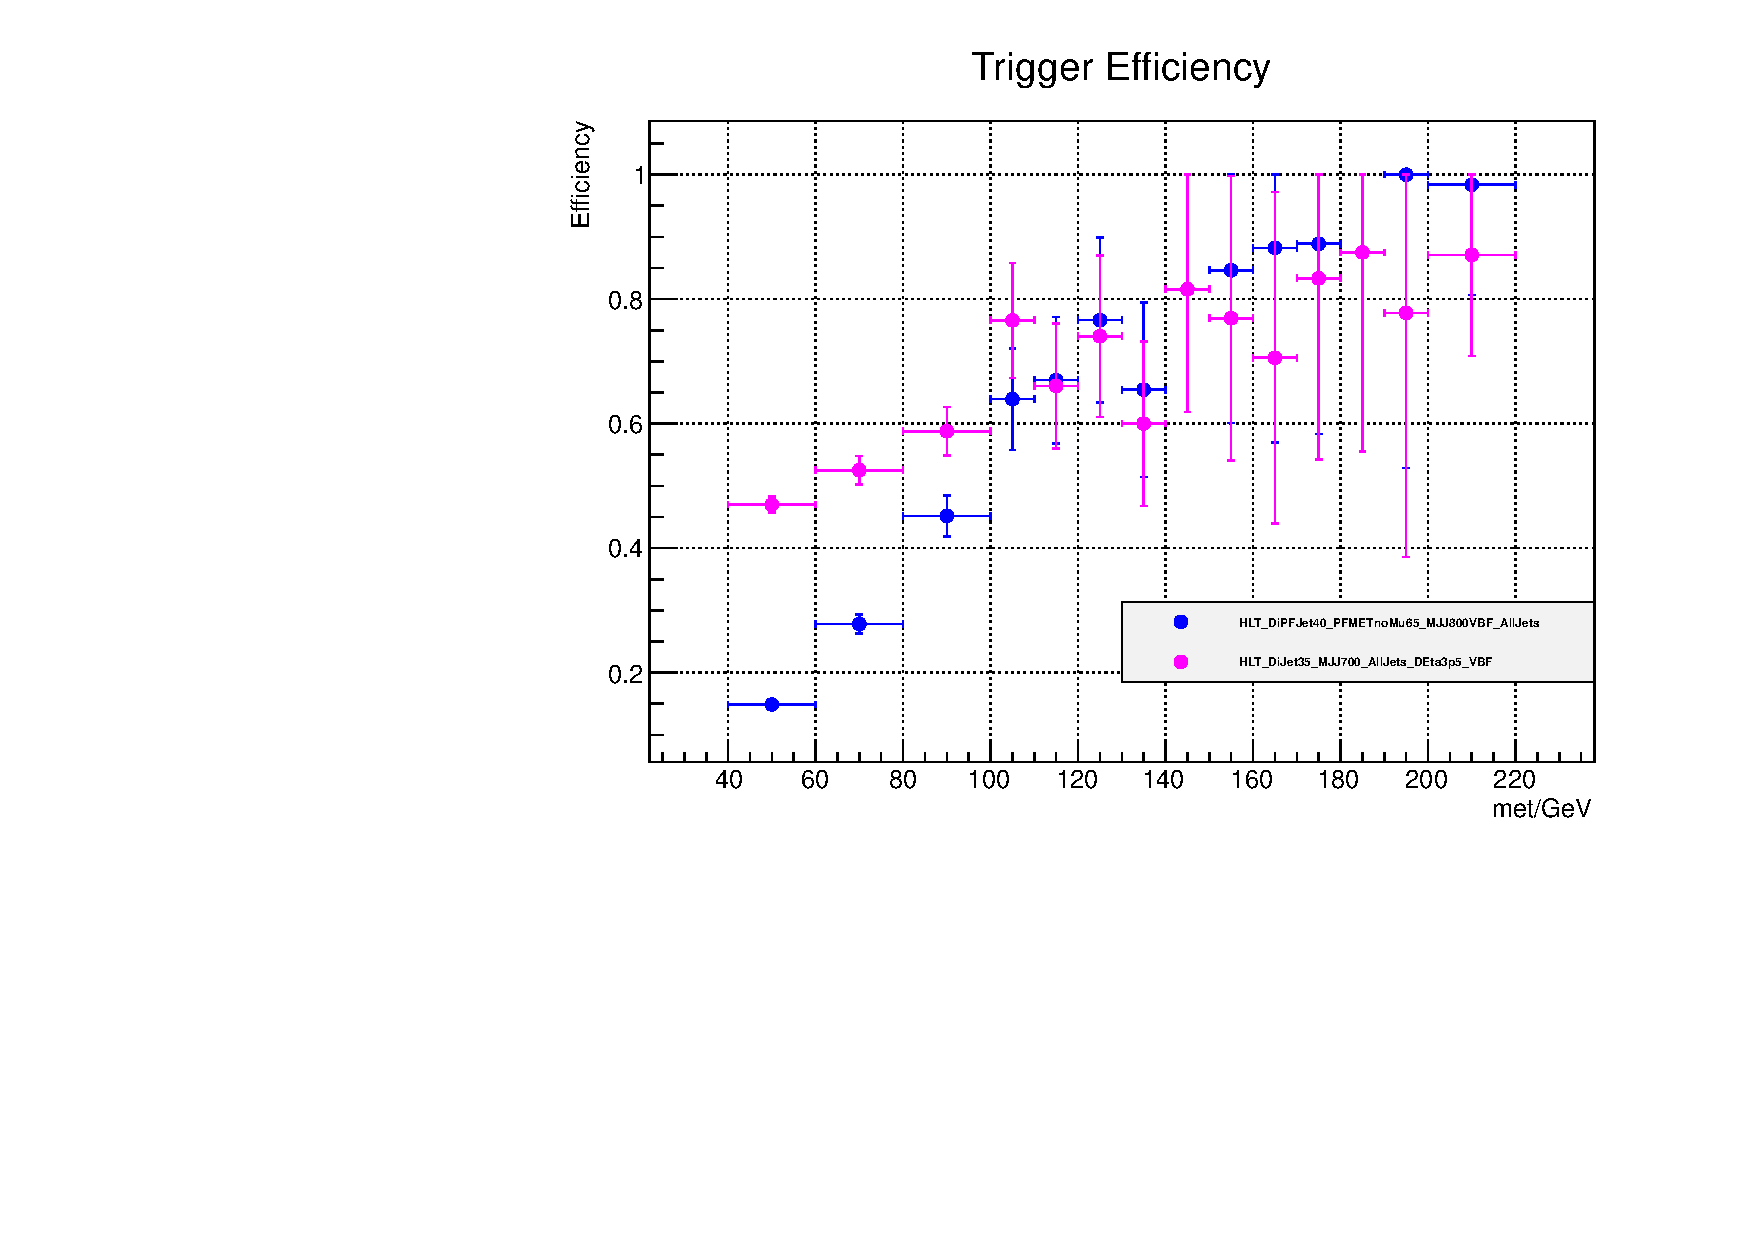
\includegraphics[width=\textwidth]{TalkPics/trigeffplots/metefficiency1.pdf}
    \end{block}
  \end{columns}
\end{frame}
\begin{frame}
  \frametitle{MET - Run by Run}
  \begin{block}{}
    \scriptsize
    \begin{itemize}
    \item All cuts except $\Delta\phi_{jj}$ and CJV have been applied
    \end{itemize}
  \end{block}
  \begin{columns}
    \column{.5\textwidth}
    \begin{block}{\scriptsize Run C}
      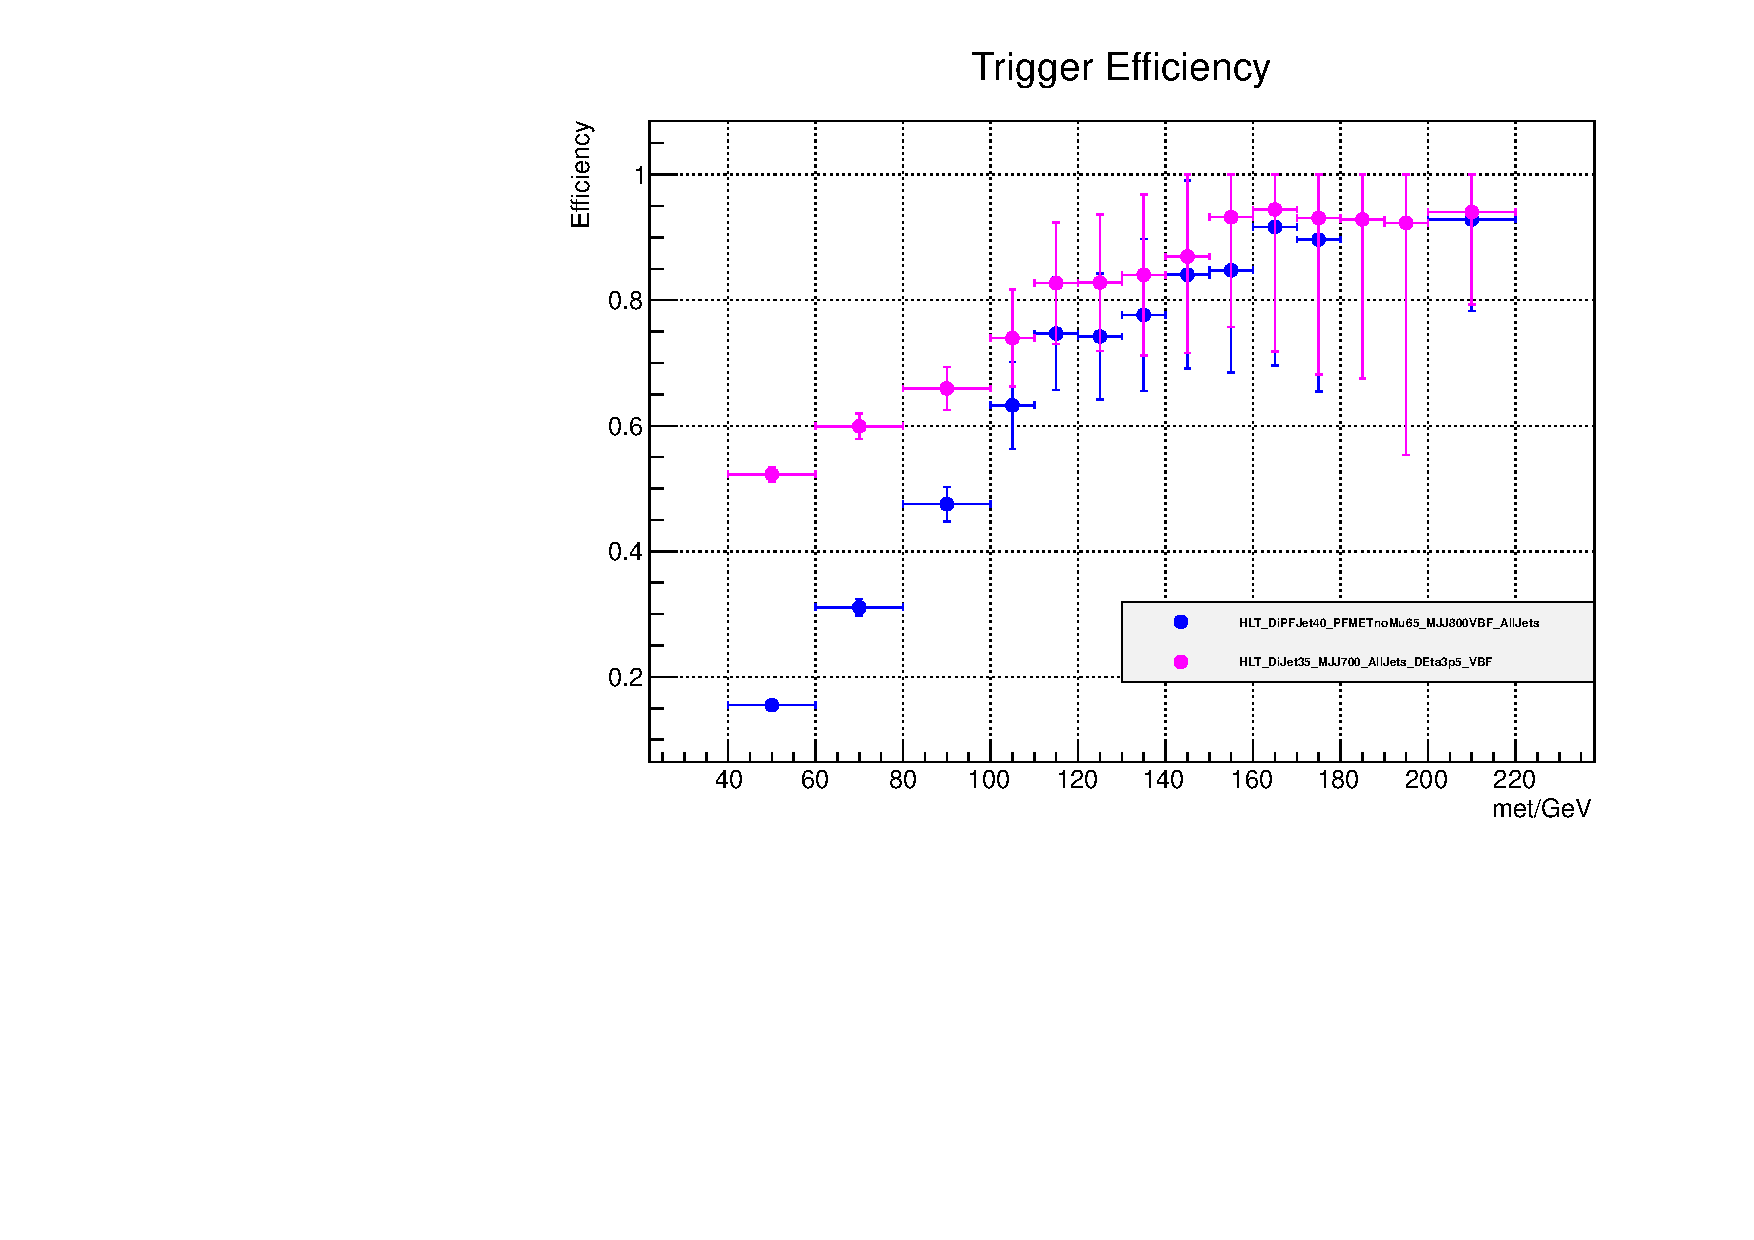
\includegraphics[width=\textwidth]{TalkPics/trigeffplots/metefficiency2.pdf}
    \end{block}
    \column{.5\textwidth}
    \begin{block}{\scriptsize Run D}
      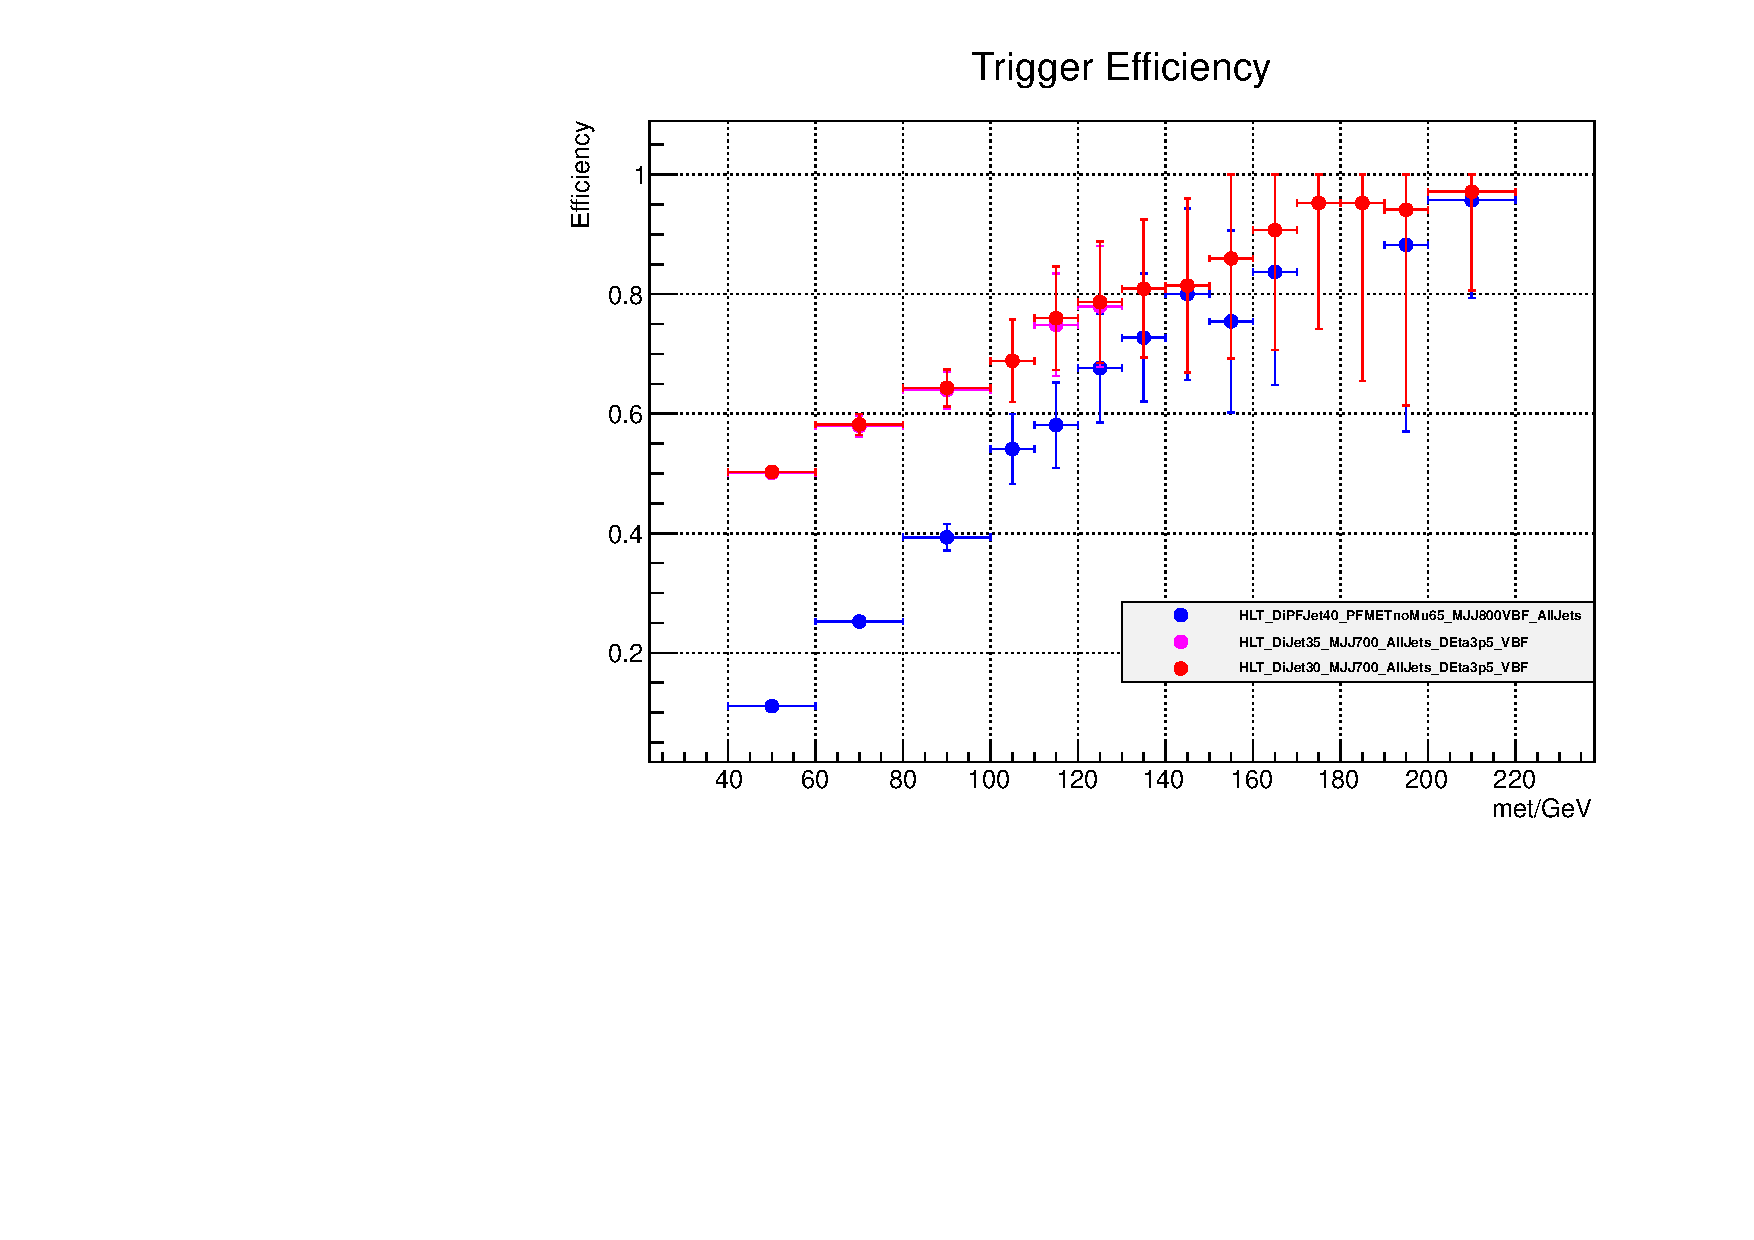
\includegraphics[width=\textwidth]{TalkPics/trigeffplots/metefficiency3.pdf}
    \end{block}
  \end{columns}
\end{frame}

\begin{frame}
  \frametitle{MET - All runs combined}
  \begin{columns}
    \column{.5\textwidth}
    \begin{block}{}
      \scriptsize
      \begin{itemize}
      \item All cuts except $\Delta\phi_{jj}$ and CJV have been applied
      \end{itemize}
    \end{block}
    
    \begin{block}{}
      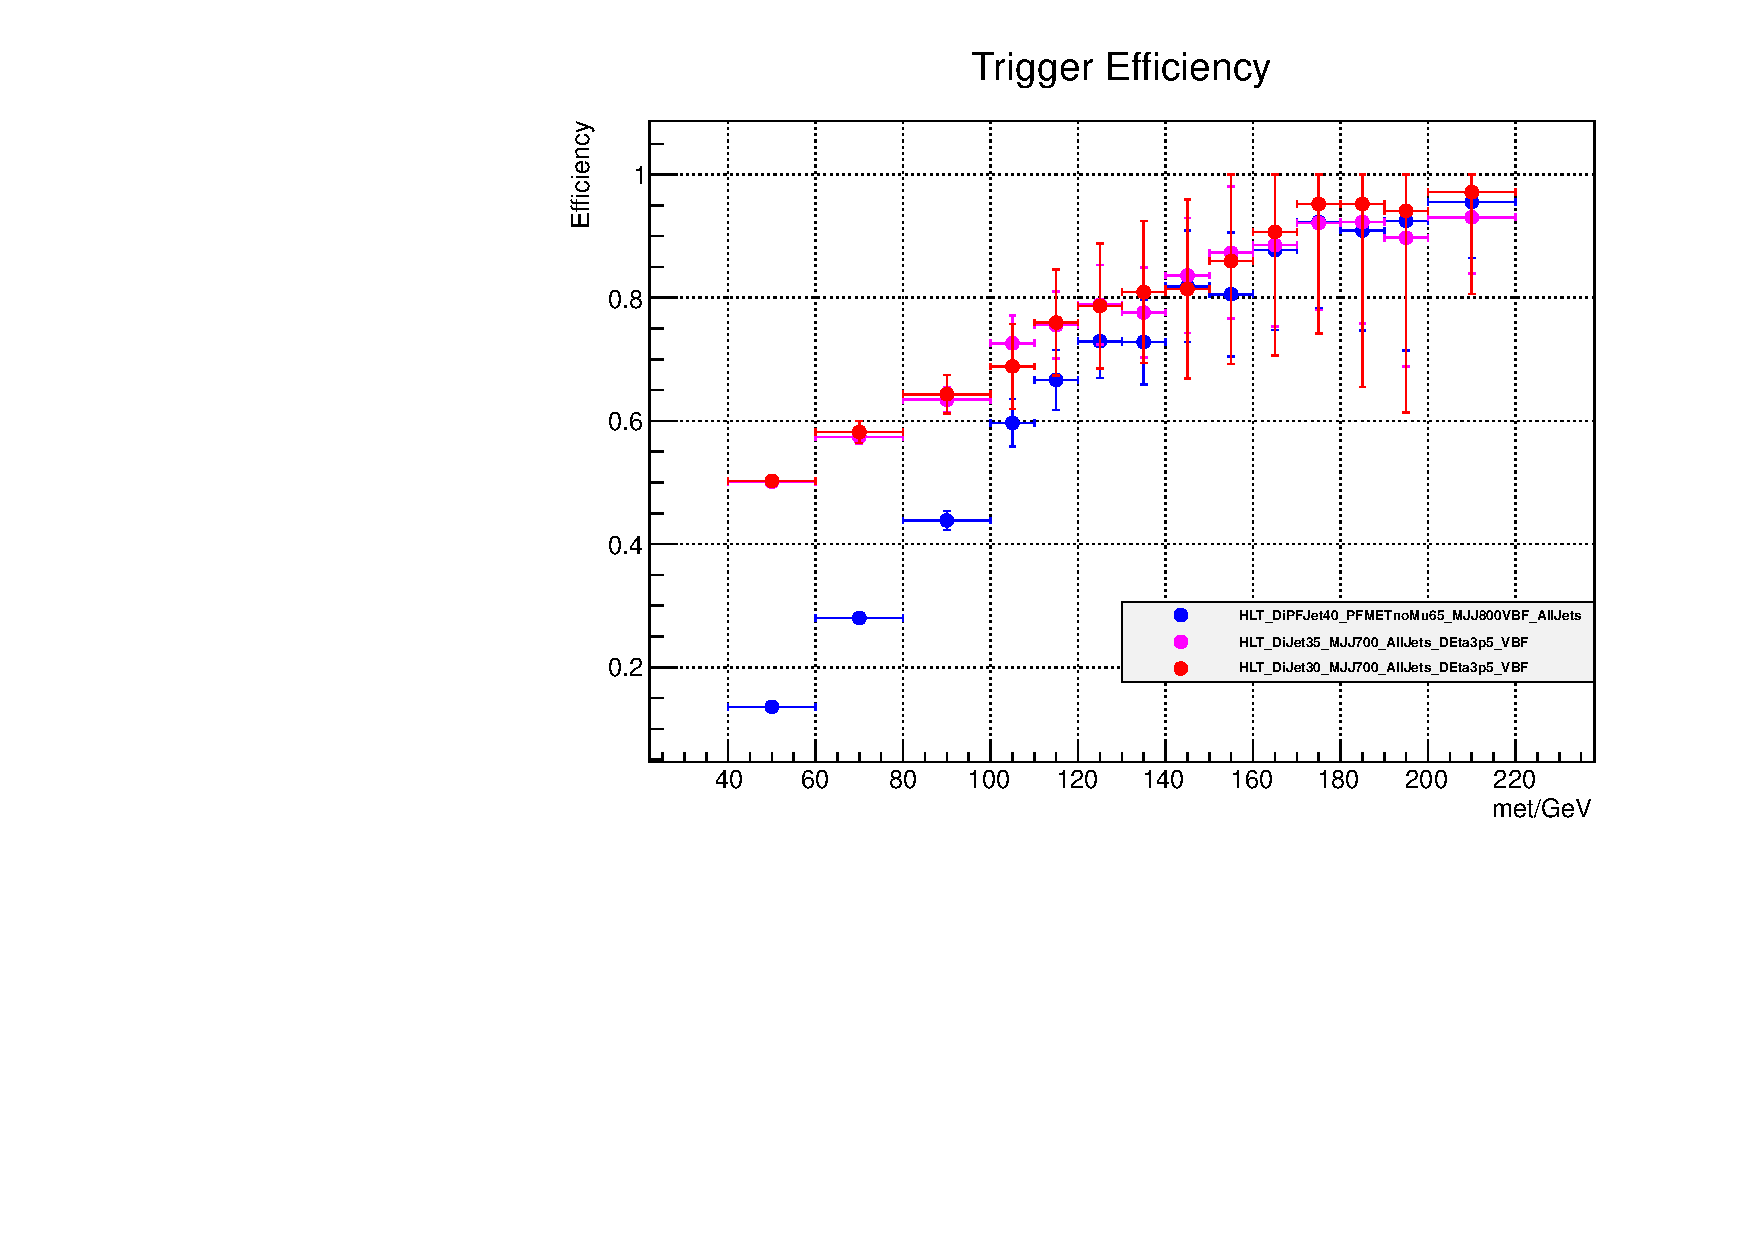
\includegraphics[width=\textwidth]{TalkPics/trigeffplots/metefficiency.pdf}
    \end{block}
    \column{.5\textwidth}
    \begin{block}{}
      \scriptsize
      \begin{itemize}
      \item All cuts have been applied
      \end{itemize}
    \end{block}
    
    \begin{block}{}
      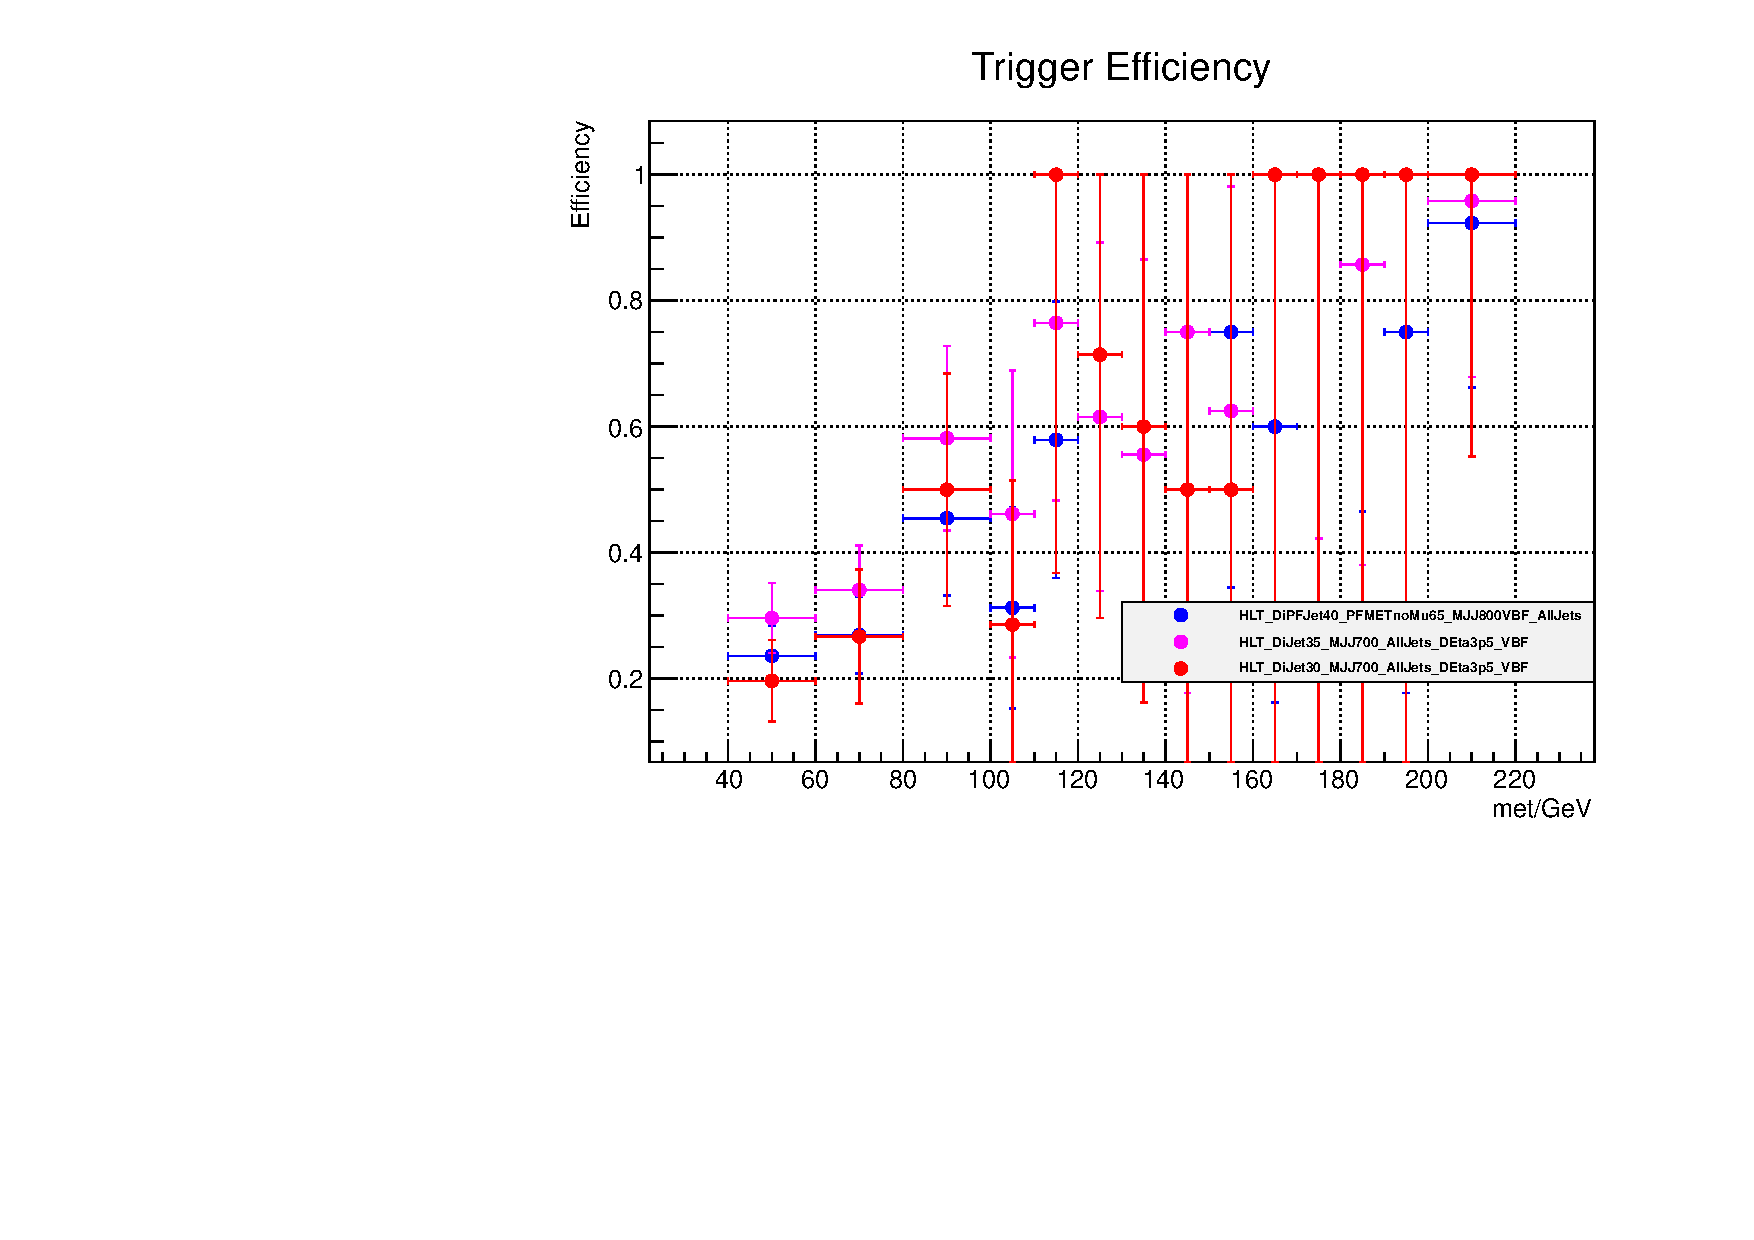
\includegraphics[width=\textwidth]{TalkPics/trigeffplotsallcuts/metefficiency.pdf}
    \end{block}
    
  \end{columns}
\end{frame}


\begin{frame}
  \frametitle{$M_{jj}$ - Run by Run}
  \begin{block}{}
    \scriptsize
    \begin{itemize}
    \item All cuts except $\Delta\phi_{jj}$ and CJV have been applied
    \end{itemize}
  \end{block}
  \begin{columns}
    \column{.5\textwidth}
    \begin{block}{\scriptsize Run A}
      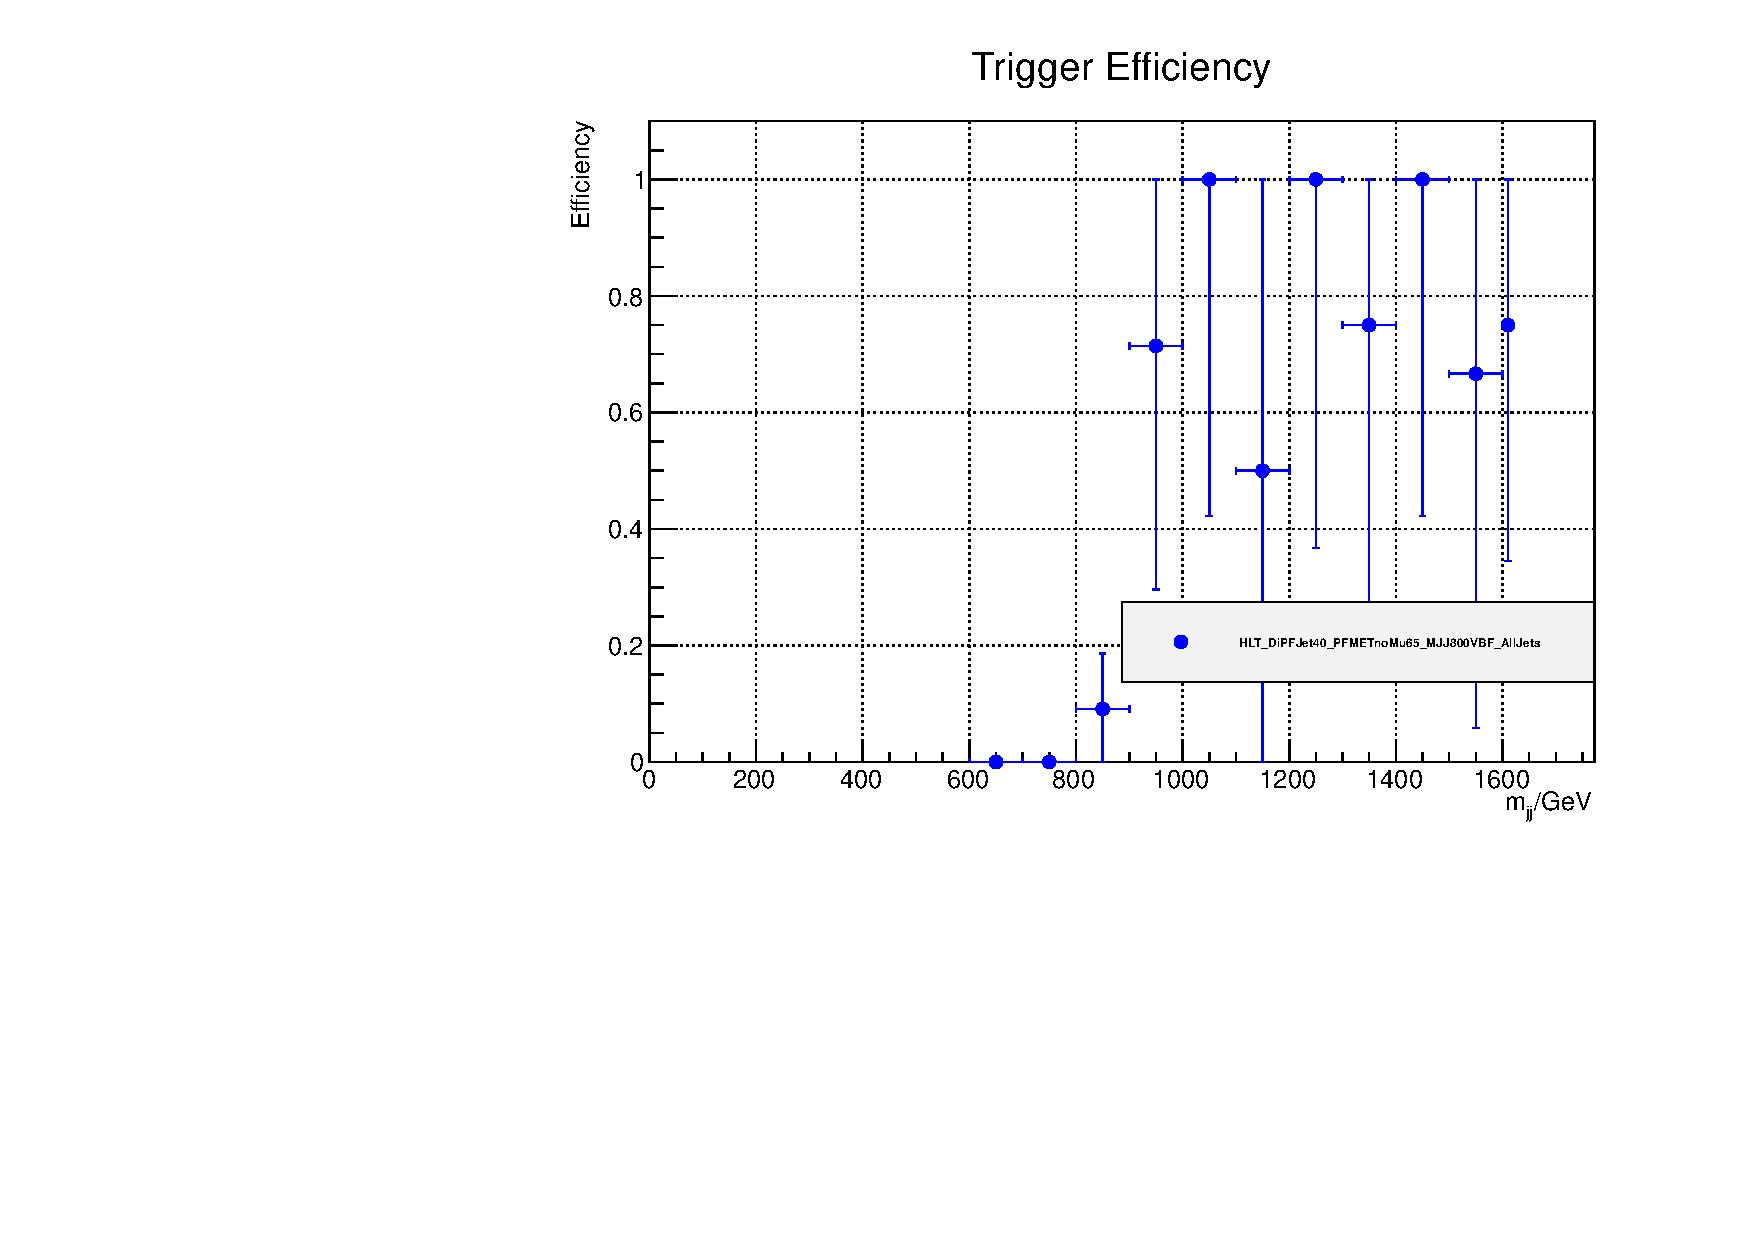
\includegraphics[width=\textwidth]{TalkPics/trigeffplots/mjjefficiency0.pdf}
    \end{block}
    \column{.5\textwidth}
    \begin{block}{\scriptsize Run B}
      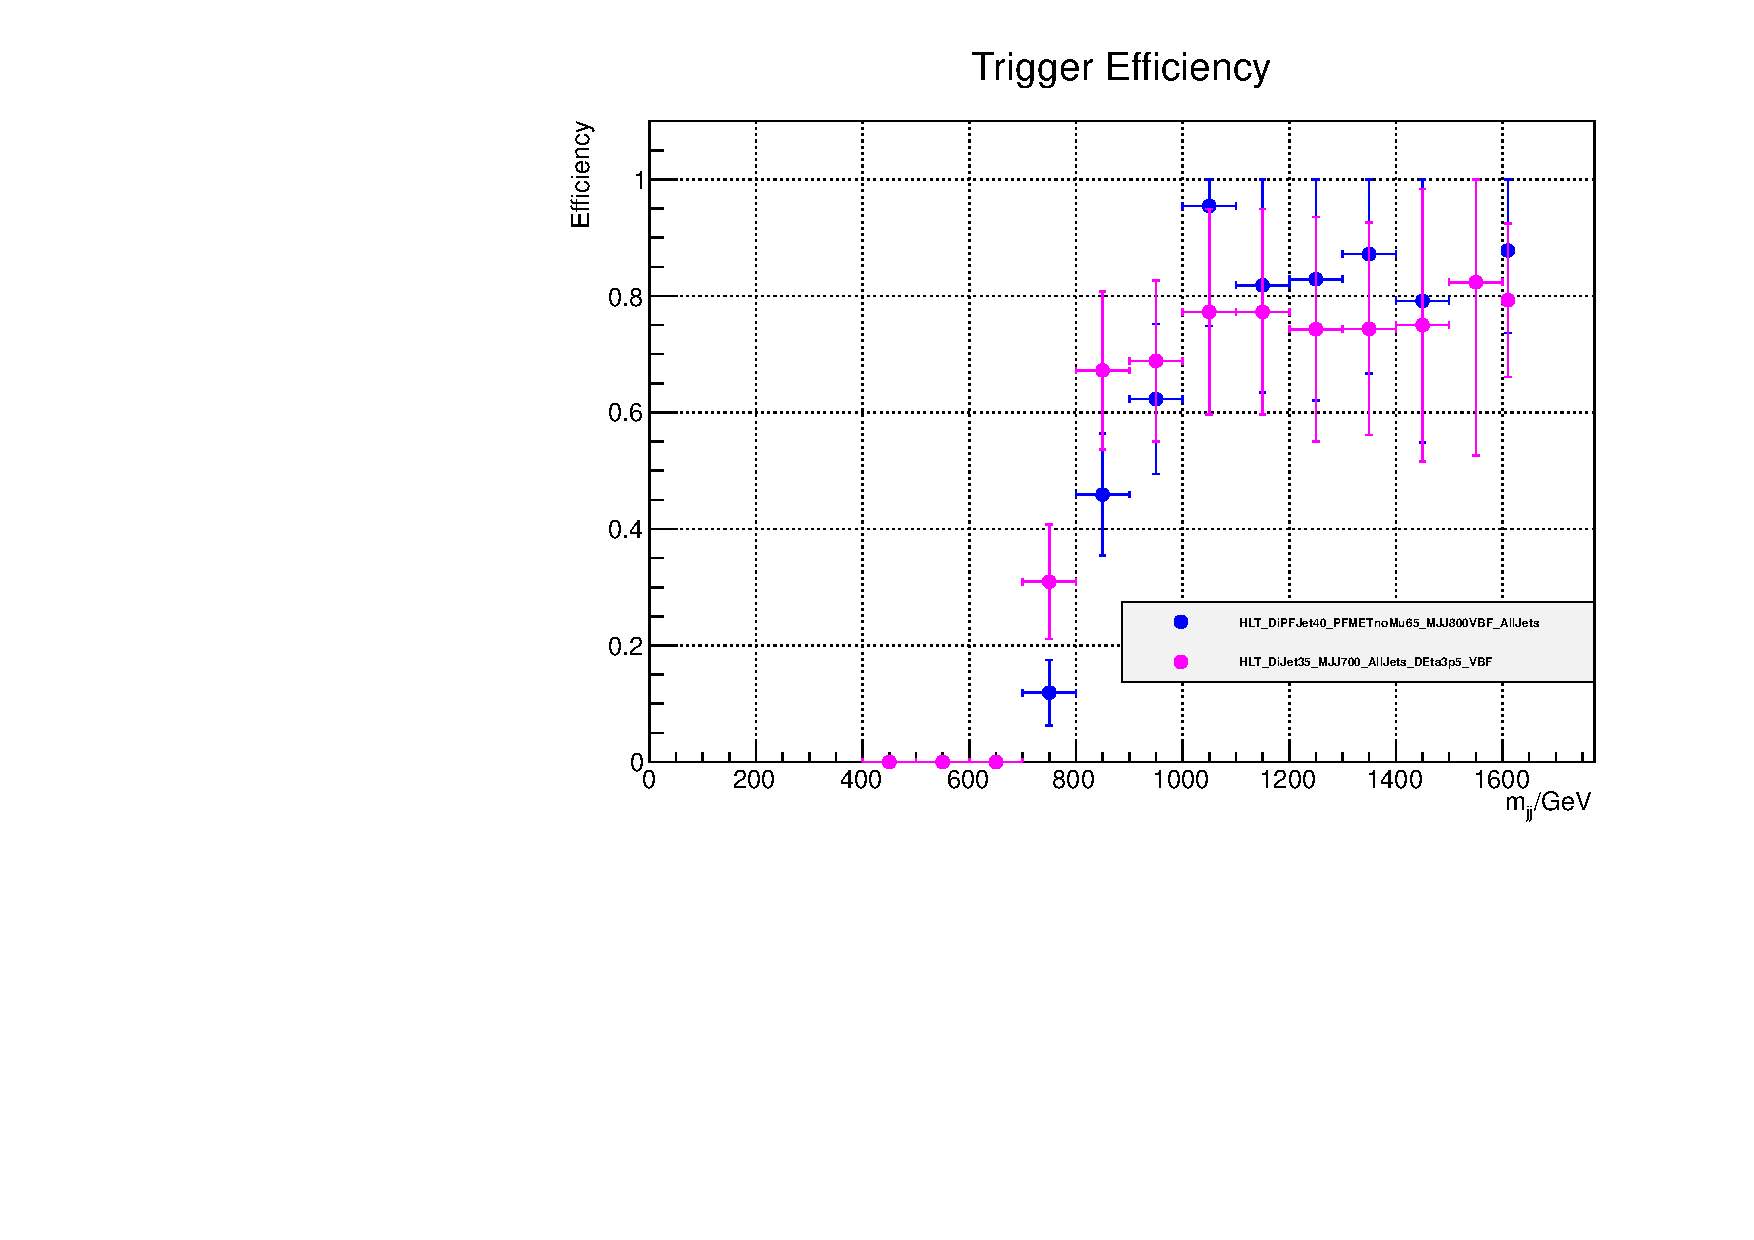
\includegraphics[width=\textwidth]{TalkPics/trigeffplots/mjjefficiency1.pdf}
    \end{block}
  \end{columns}
\end{frame}
\begin{frame}
  \frametitle{$M_{jj}$ - Run by Run}
  \begin{block}{}
    \scriptsize
    \begin{itemize}
    \item All cuts except $\Delta\phi_{jj}$ and CJV have been applied
    \end{itemize}
  \end{block}
  \begin{columns}
    \column{.5\textwidth}
    \begin{block}{\scriptsize Run C}
      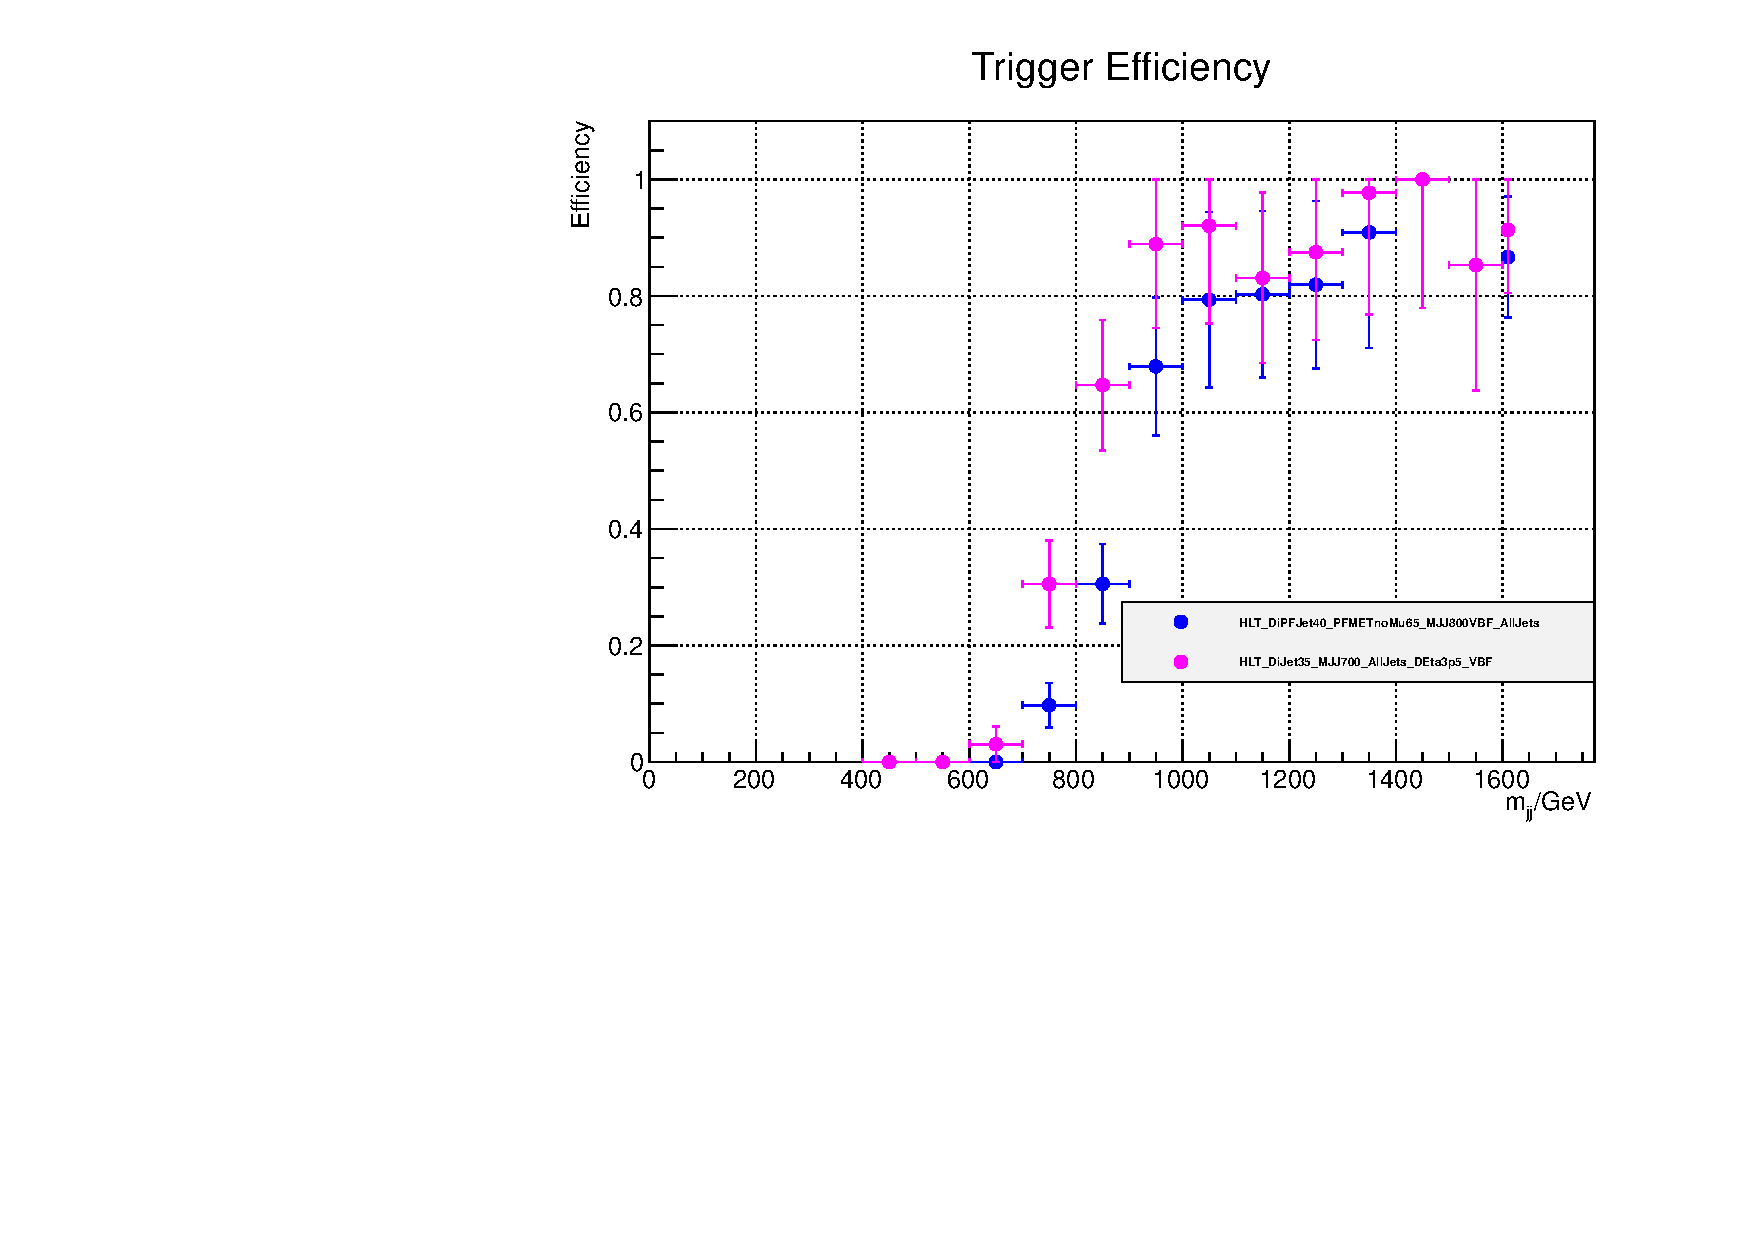
\includegraphics[width=\textwidth]{TalkPics/trigeffplots/mjjefficiency2.pdf}
    \end{block}
    \column{.5\textwidth}
    \begin{block}{\scriptsize Run D}
      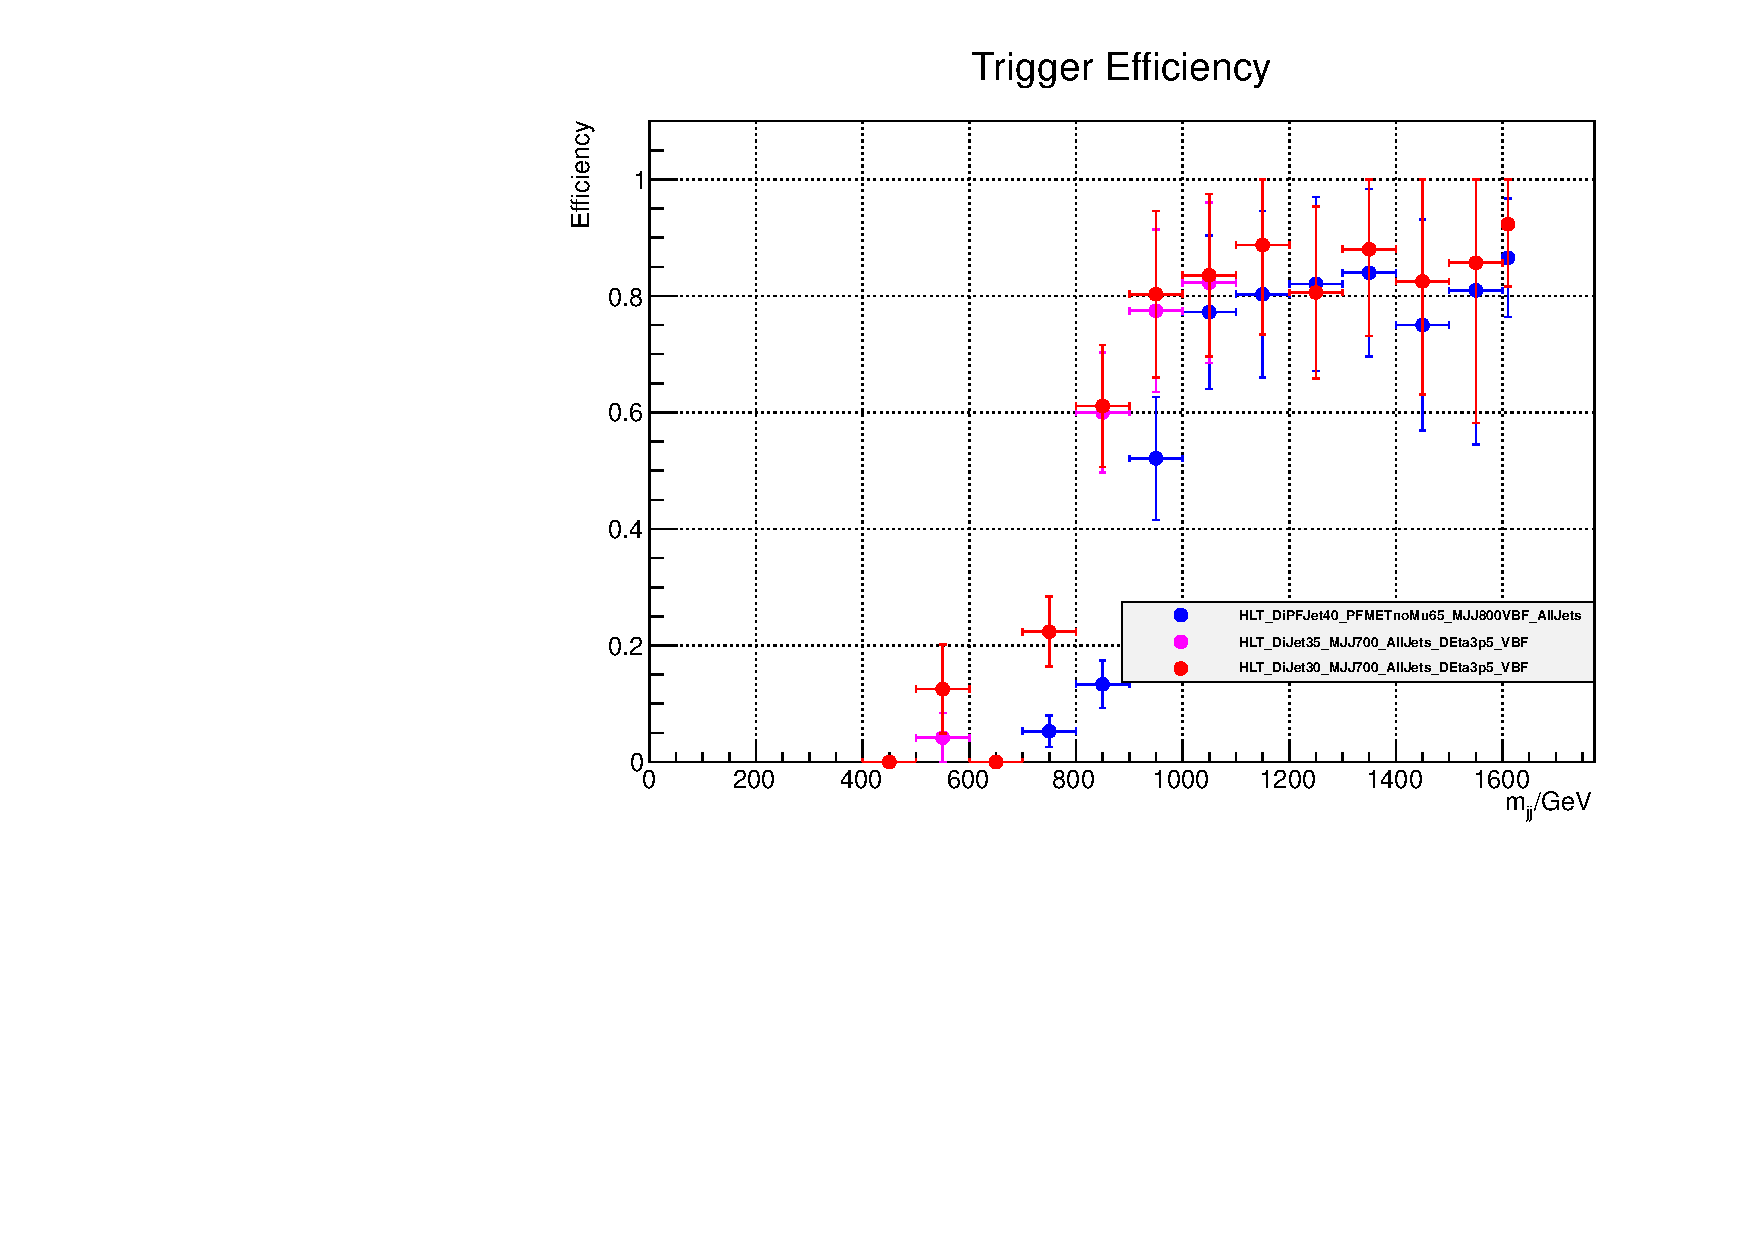
\includegraphics[width=\textwidth]{TalkPics/trigeffplots/mjjefficiency3.pdf}
    \end{block}
  \end{columns}
\end{frame}


\begin{frame}
  \frametitle{$M_{jj}$  - All runs combined}
  \begin{columns}
    \column{.5\textwidth}
    \begin{block}{}
      \scriptsize
      \begin{itemize}
      \item All cuts except $\Delta\phi_{jj}$ and CJV have been applied
      \end{itemize}
    \end{block}
    
    \begin{block}{}
      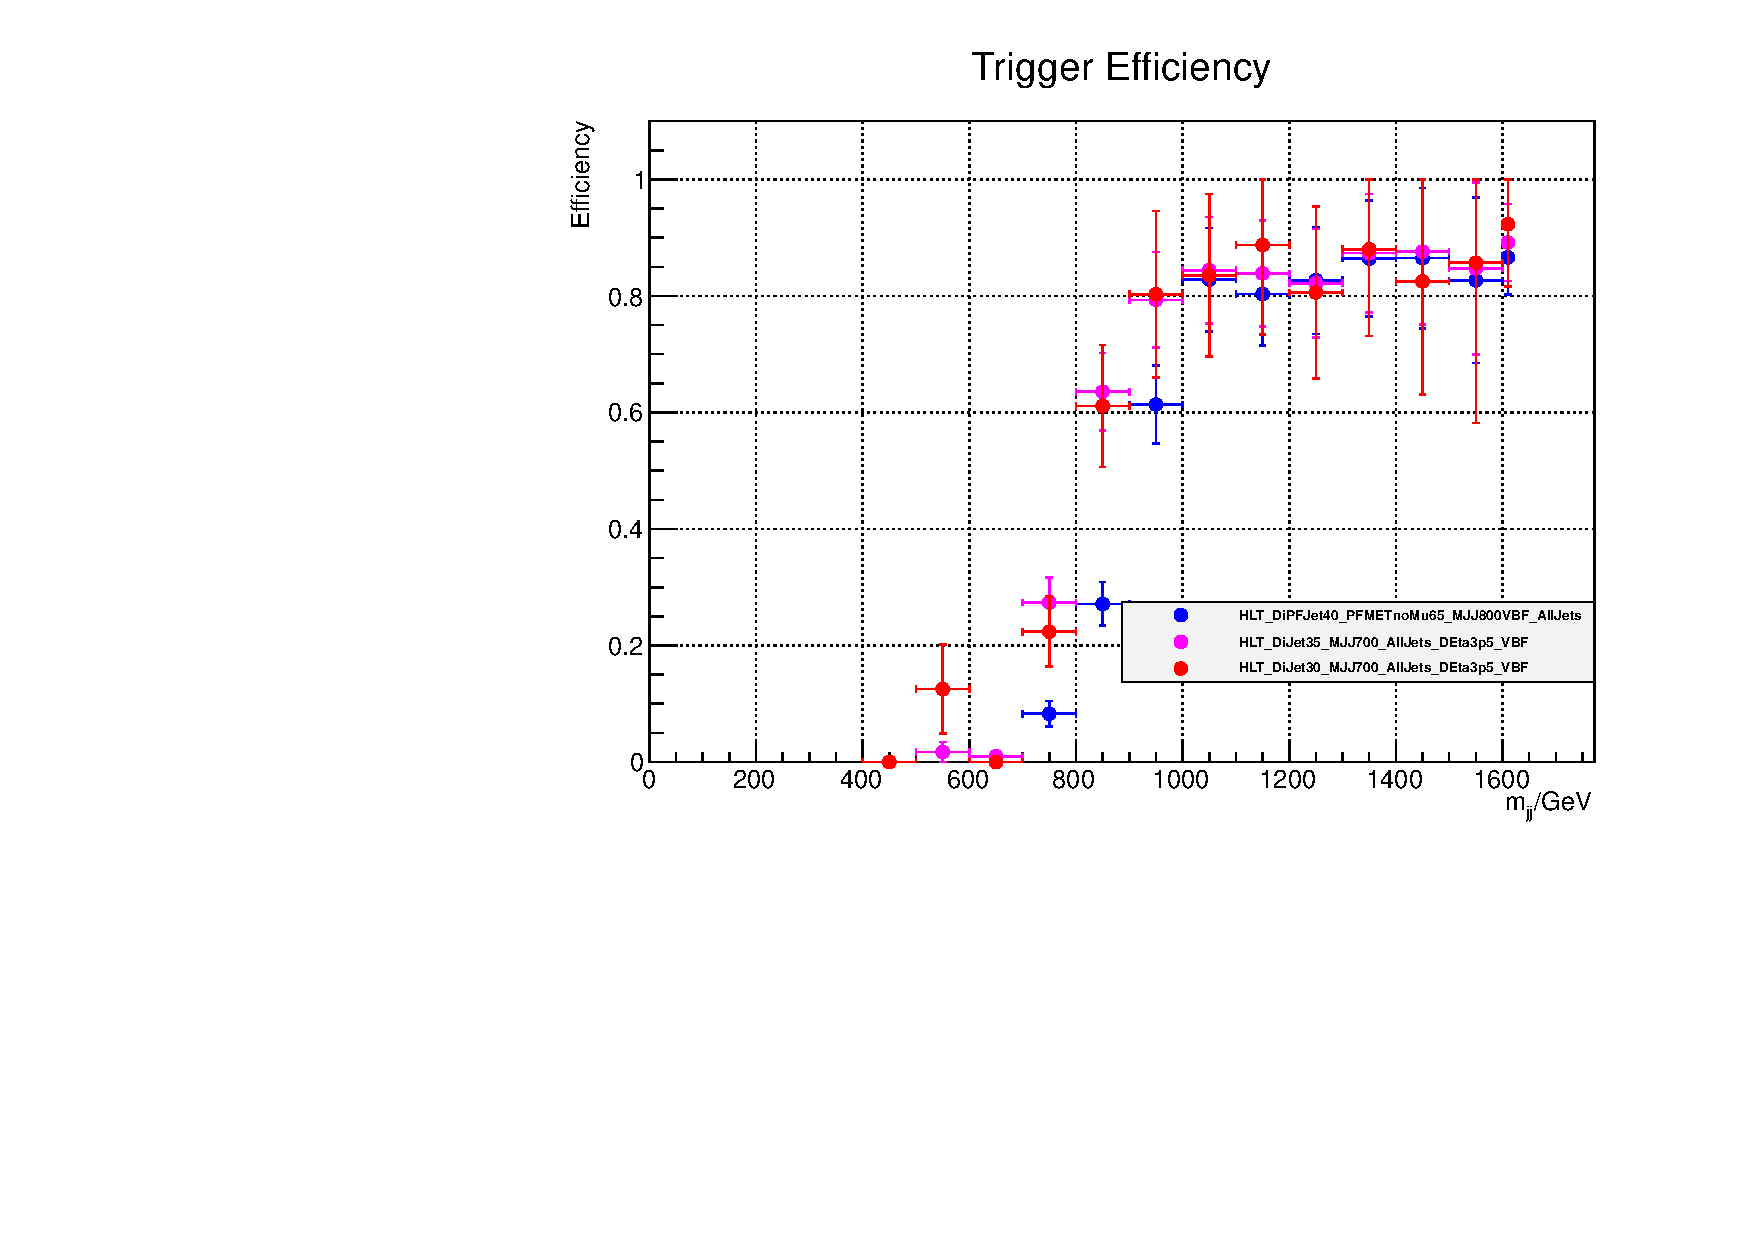
\includegraphics[width=\textwidth]{TalkPics/trigeffplots/mjjefficiency.pdf}
    \end{block}

    \column{.5\textwidth}
    \begin{block}{}
      \scriptsize
      \begin{itemize}
      \item All cuts have been applied
      \end{itemize}
    \end{block}
    
    \begin{block}{}
      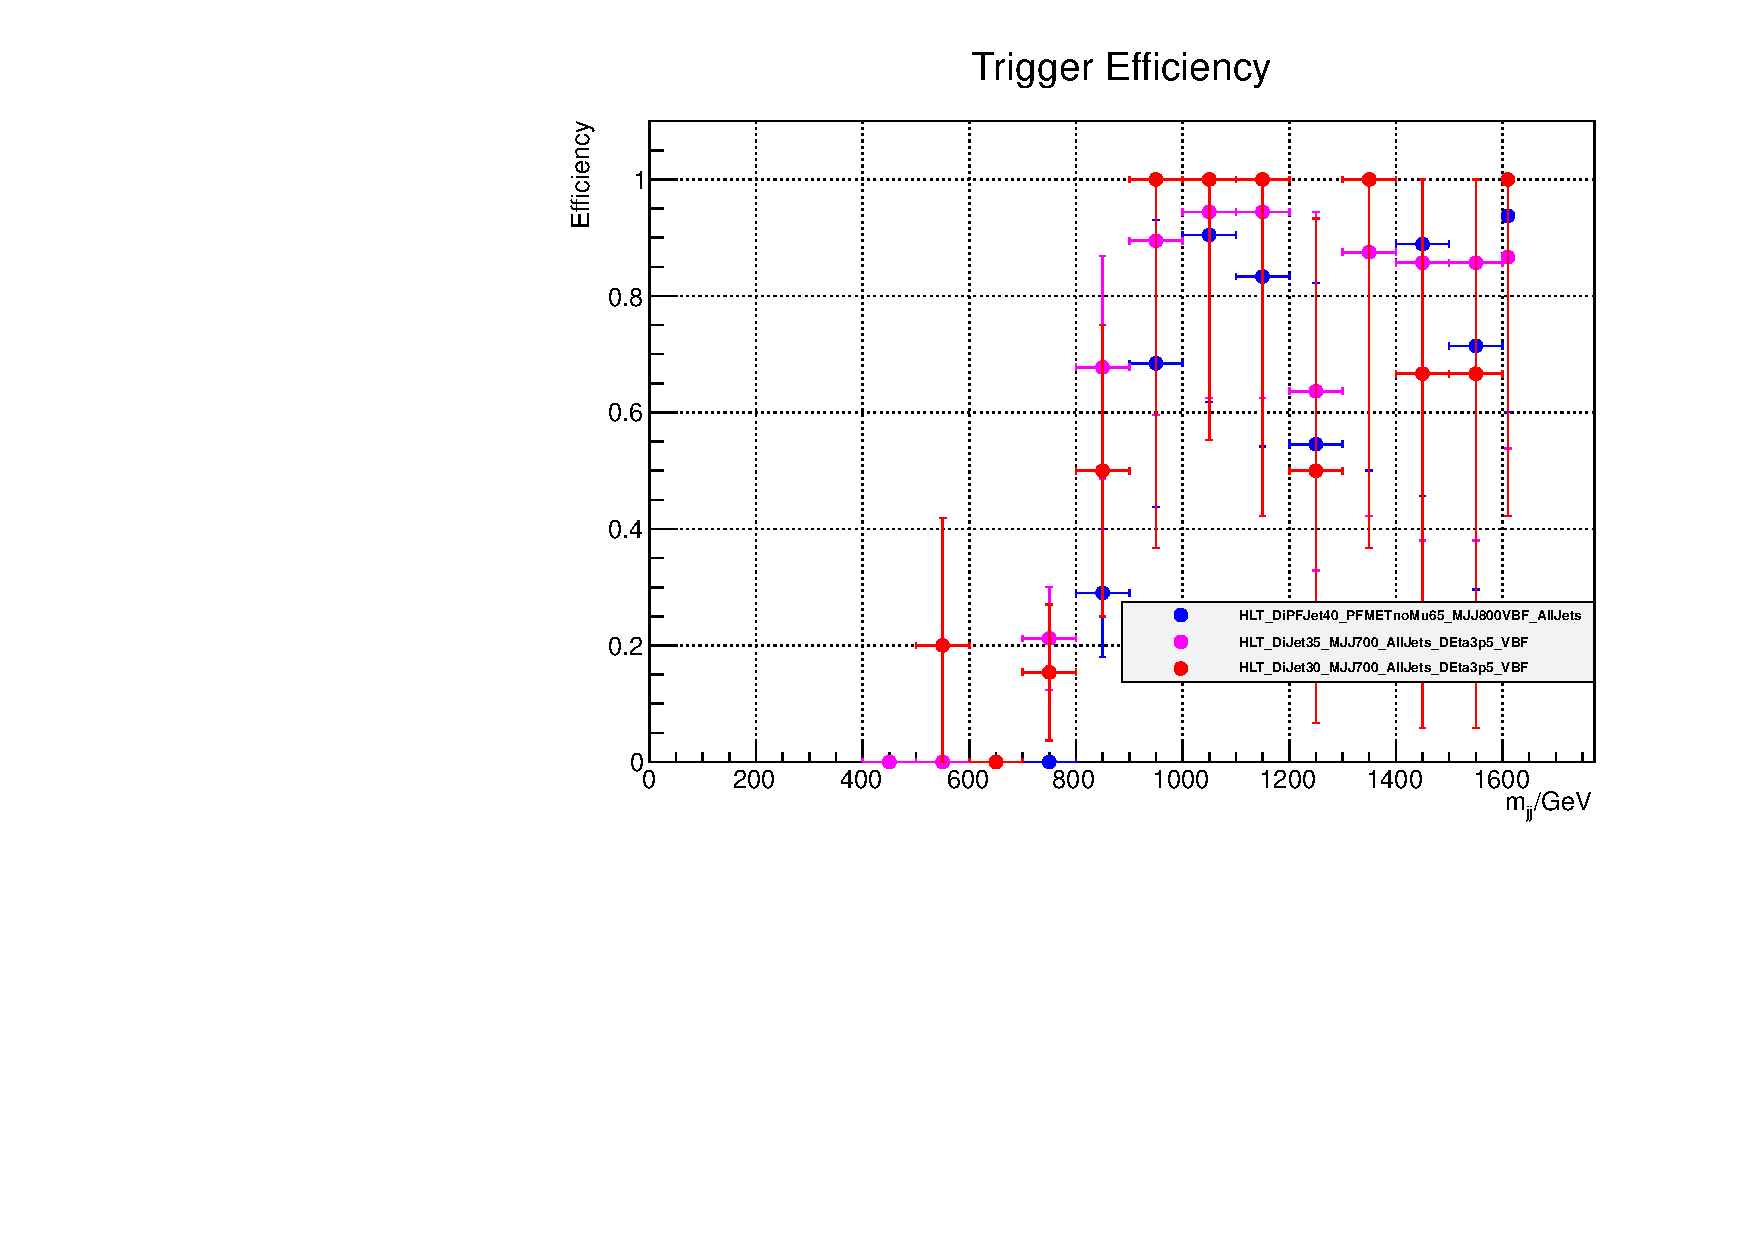
\includegraphics[width=\textwidth]{TalkPics/trigeffplotsallcuts/mjjefficiency.pdf}
    \end{block}

  \end{columns}
\end{frame}

\begin{frame}
  \frametitle{Jet 2 pt - Run by Run}
  \begin{block}{}
    \scriptsize
    \begin{itemize}
    \item All cuts except $\Delta\phi_{jj}$ and CJV have been applied
    \end{itemize}
  \end{block}
  \begin{columns}
    \column{.5\textwidth}
    \begin{block}{\scriptsize Run A}
      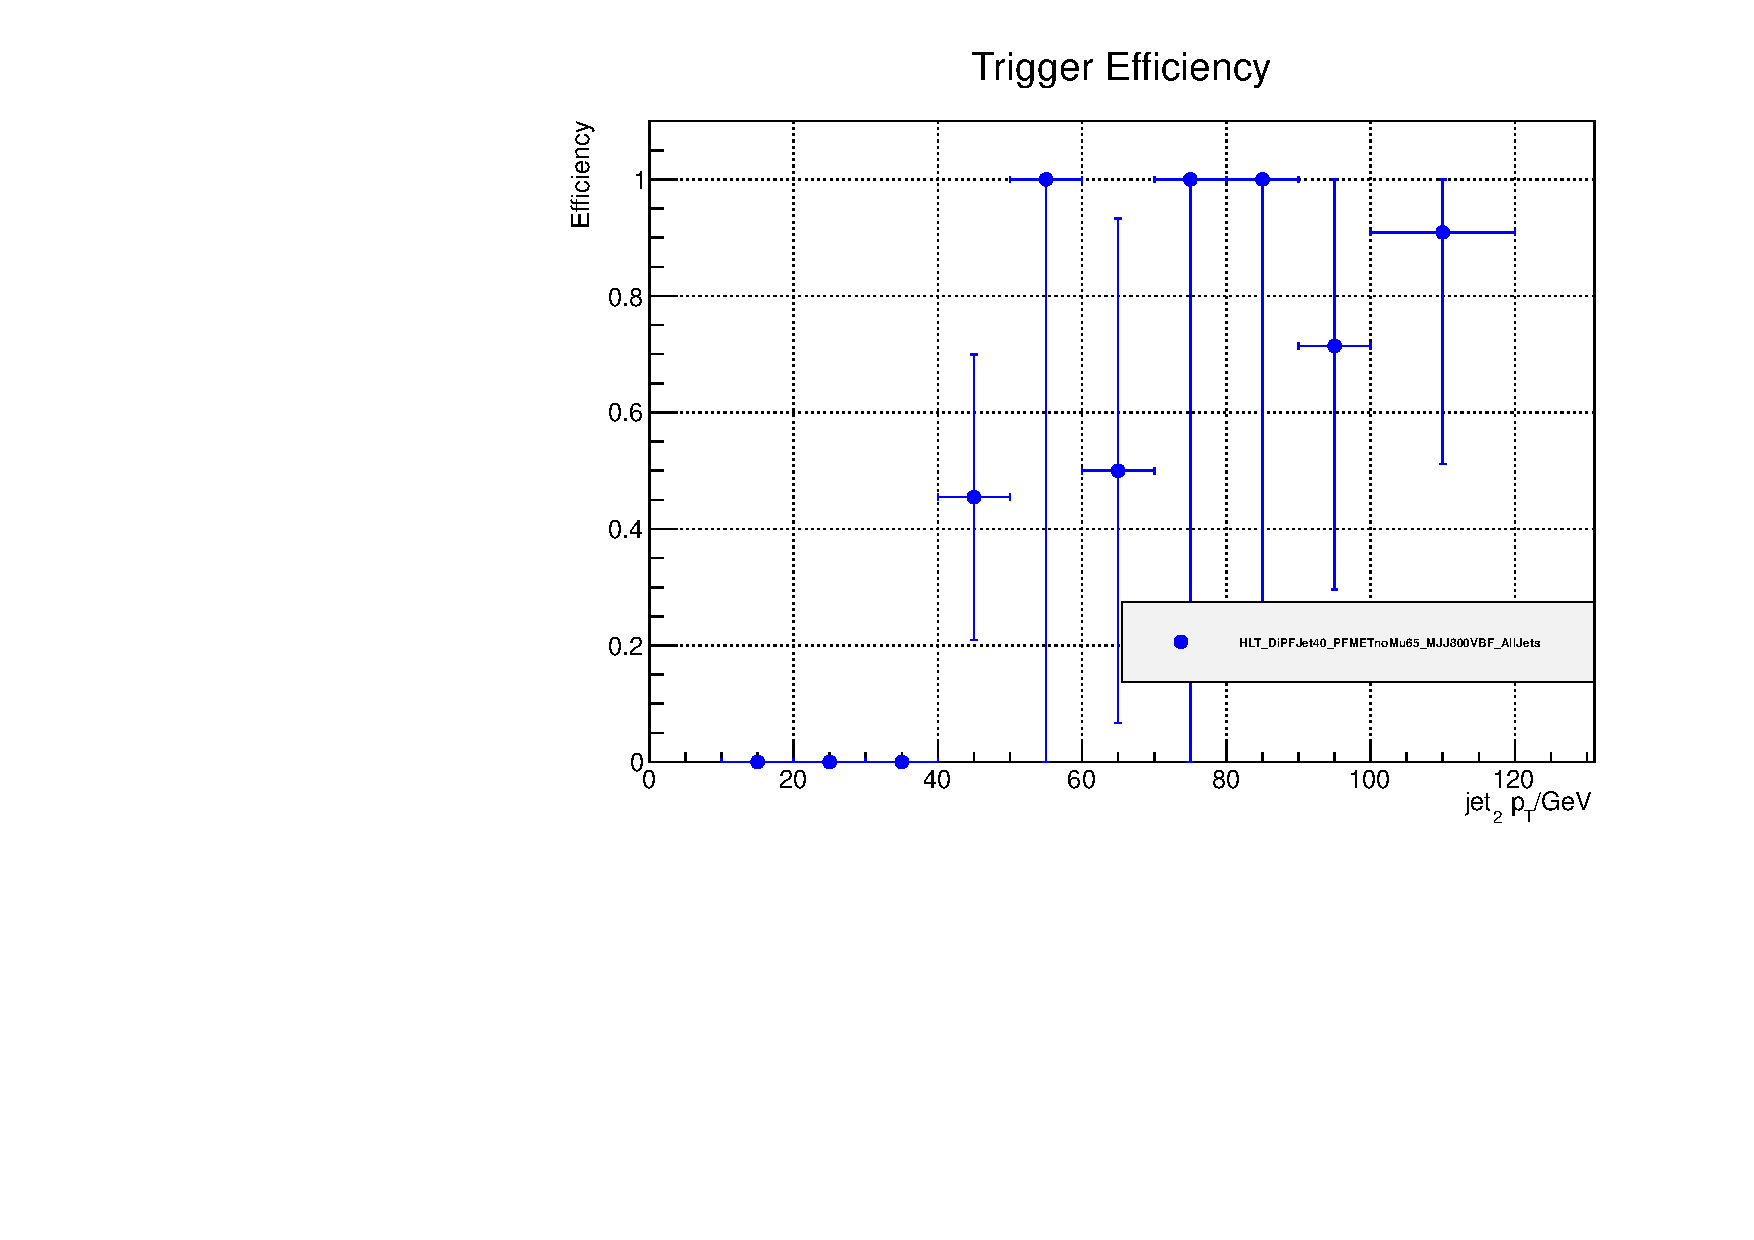
\includegraphics[width=\textwidth]{TalkPics/trigeffplots/j2ptefficiency0.pdf}
    \end{block}
    \column{.5\textwidth}
    \begin{block}{\scriptsize Run B}
      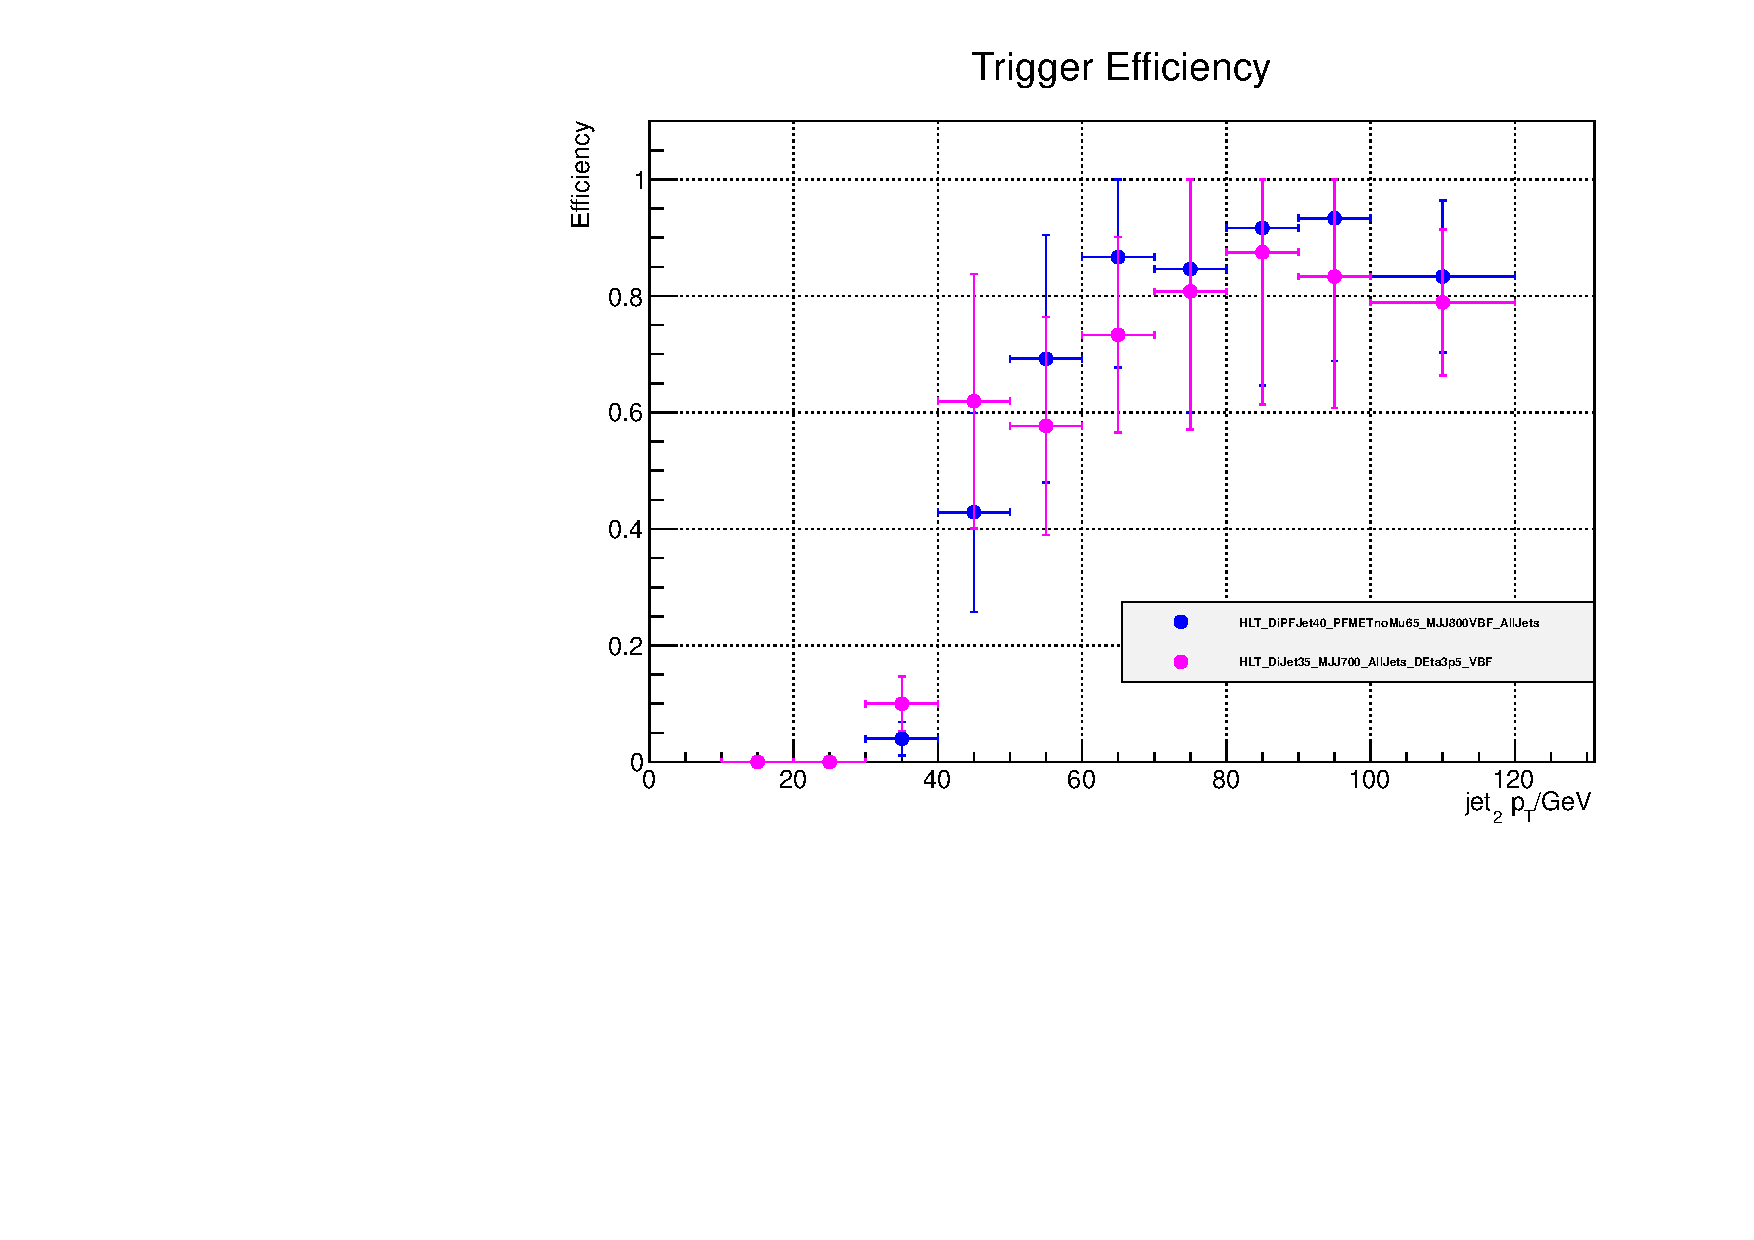
\includegraphics[width=\textwidth]{TalkPics/trigeffplots/j2ptefficiency1.pdf}
    \end{block}
  \end{columns}
\end{frame}
\begin{frame}
  \frametitle{Jet 2 pt - Run by Run}
  \begin{block}{}
    \scriptsize
    \begin{itemize}
    \item All cuts except $\Delta\phi_{jj}$ and CJV have been applied
    \end{itemize}
  \end{block}
  \begin{columns}
    \column{.5\textwidth}
    \begin{block}{\scriptsize Run C}
      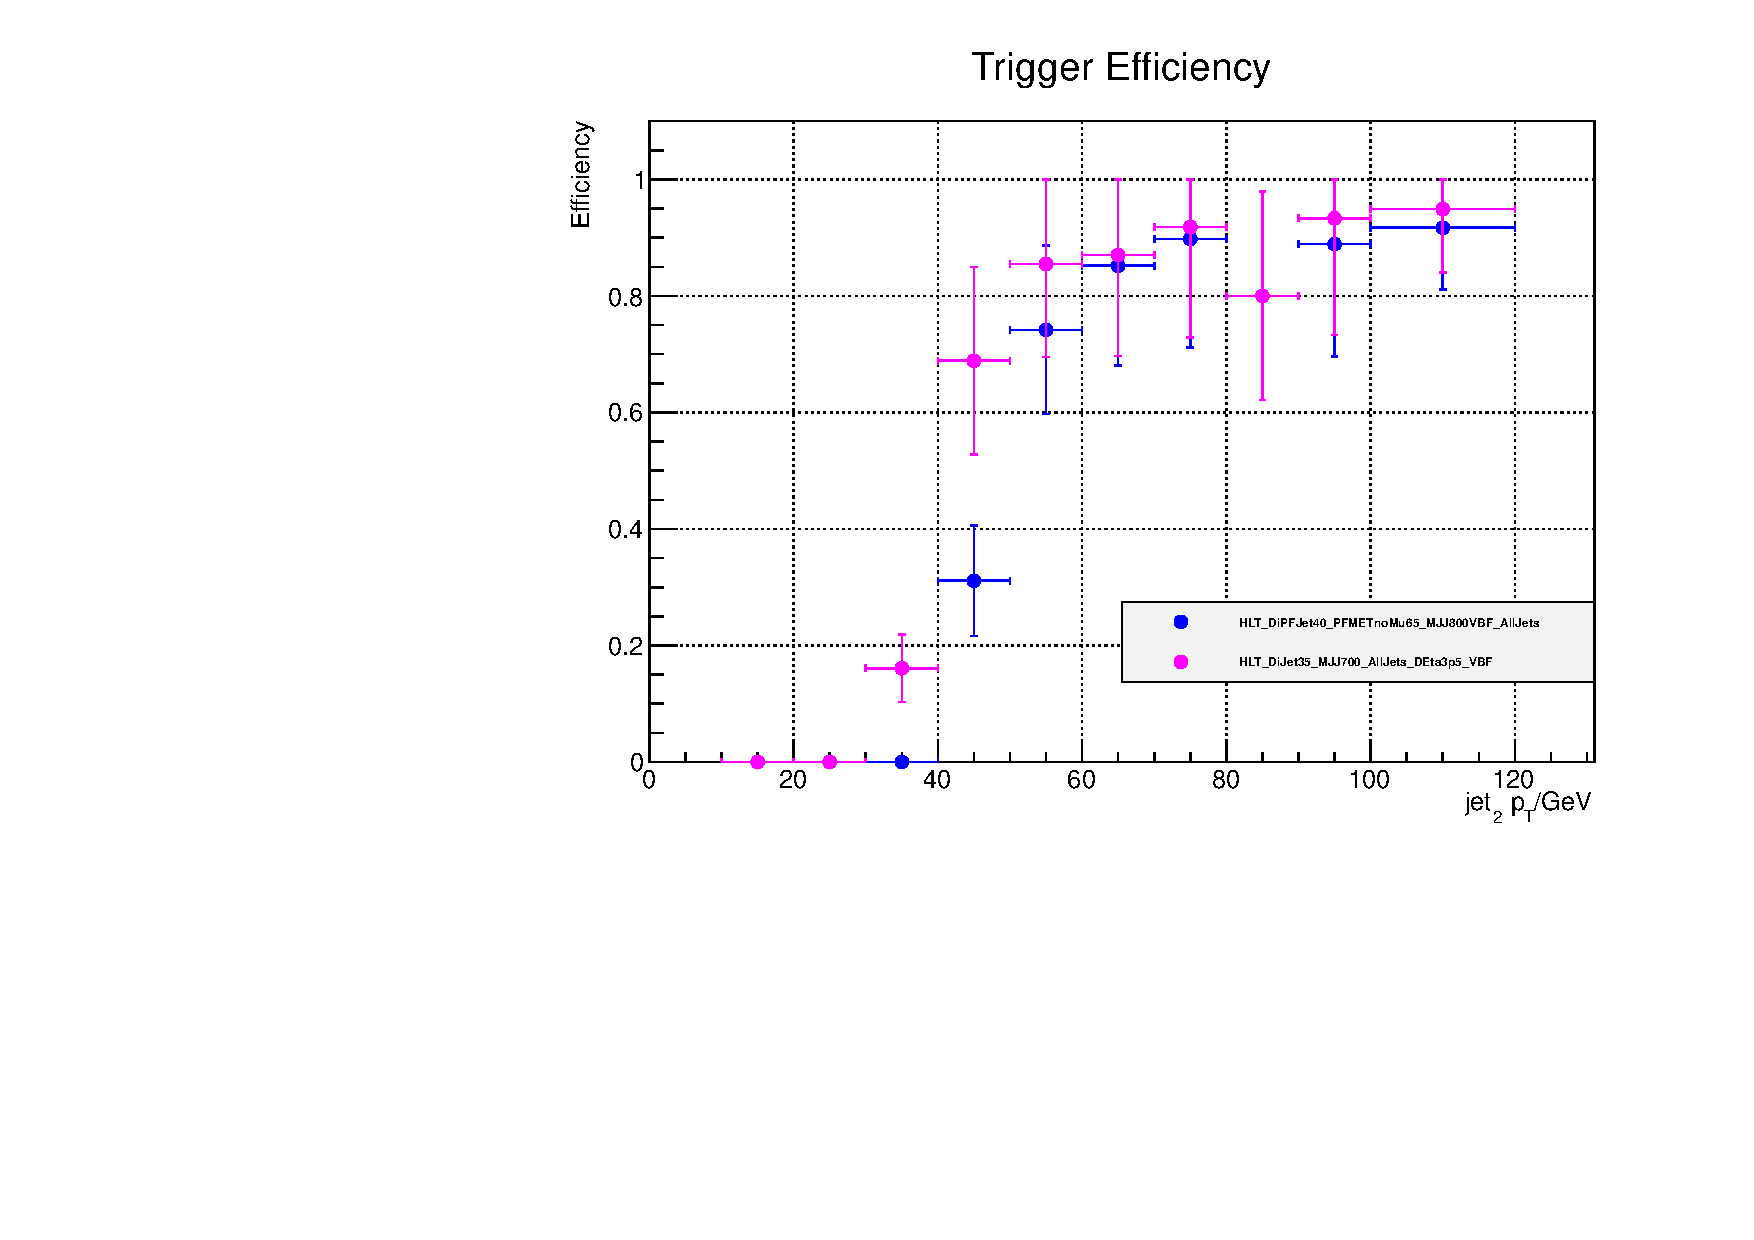
\includegraphics[width=\textwidth]{TalkPics/trigeffplots/j2ptefficiency2.pdf}
    \end{block}
    \column{.5\textwidth}
    \begin{block}{\scriptsize Run D}
      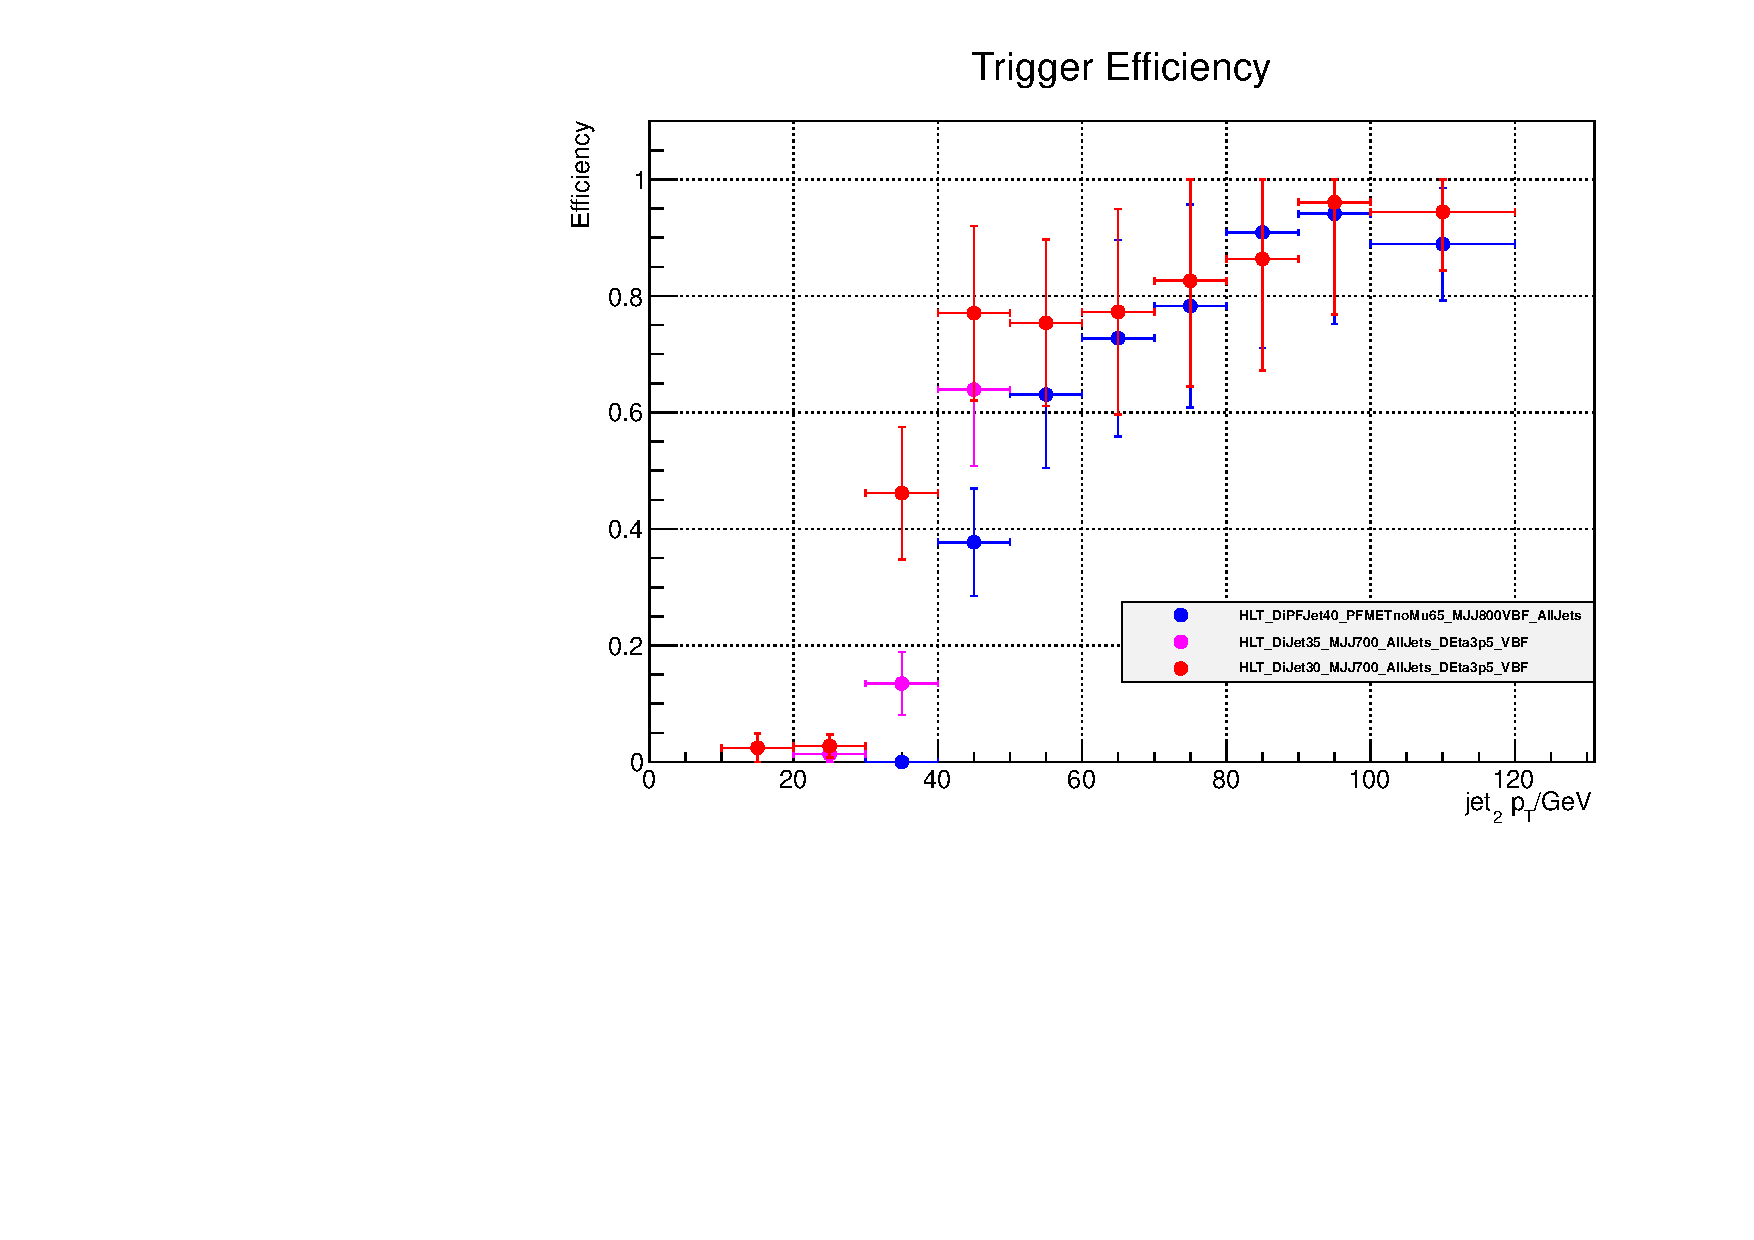
\includegraphics[width=\textwidth]{TalkPics/trigeffplots/j2ptefficiency3.pdf}
    \end{block}
  \end{columns}
\end{frame}

\begin{frame}
  \frametitle{Jet 2 pt  - All runs combined}
    \begin{columns}
      \column{.5\textwidth}
      
      \begin{block}{}
        \scriptsize
        \begin{itemize}
        \item All cuts except $\Delta\phi_{jj}$ and CJV have been applied
        \end{itemize}
      \end{block}
      \begin{block}{}
        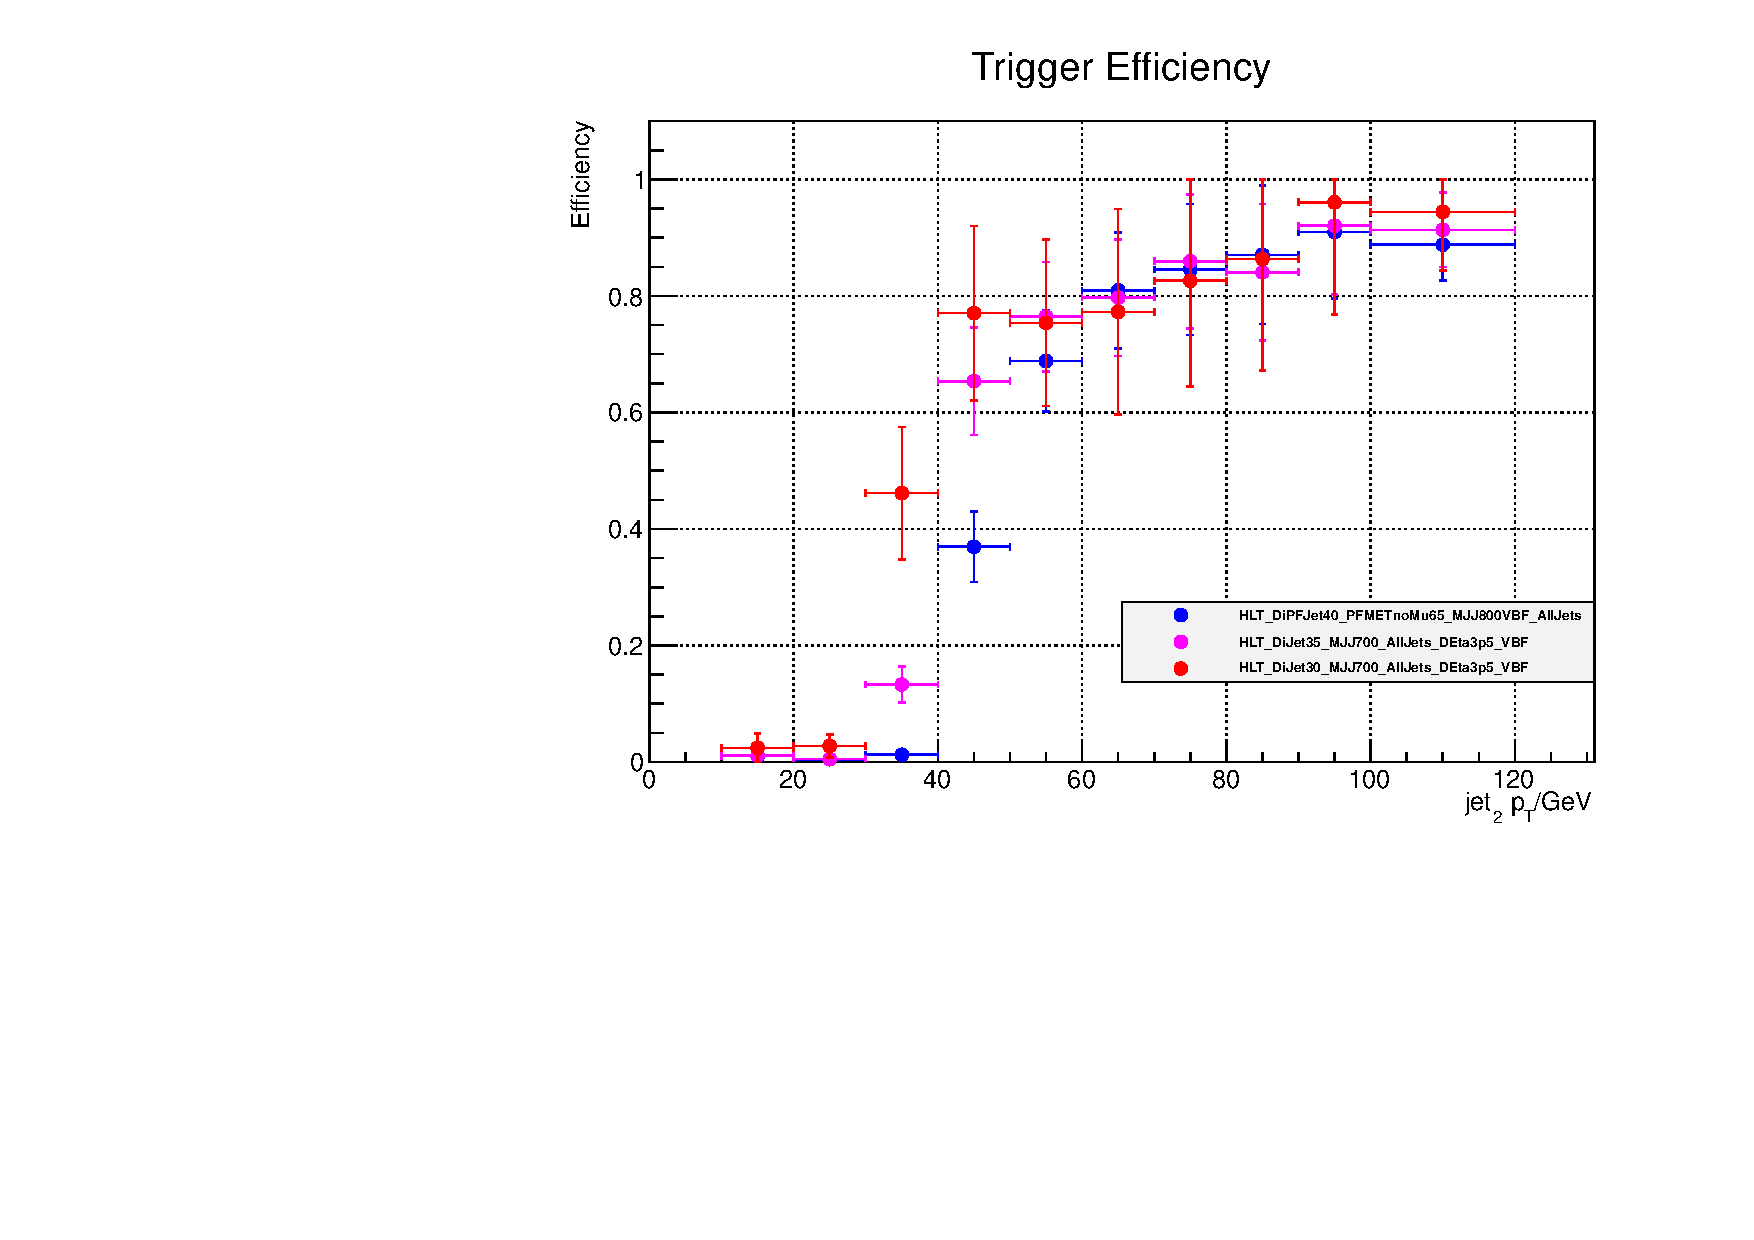
\includegraphics[width=\textwidth]{TalkPics/trigeffplots/j2ptefficiency.pdf}
      \end{block}

      \column{.5\textwidth}
      
      \begin{block}{}
        \scriptsize
        \begin{itemize}
        \item All cuts have been applied
        \end{itemize}
      \end{block}
      \begin{block}{}
        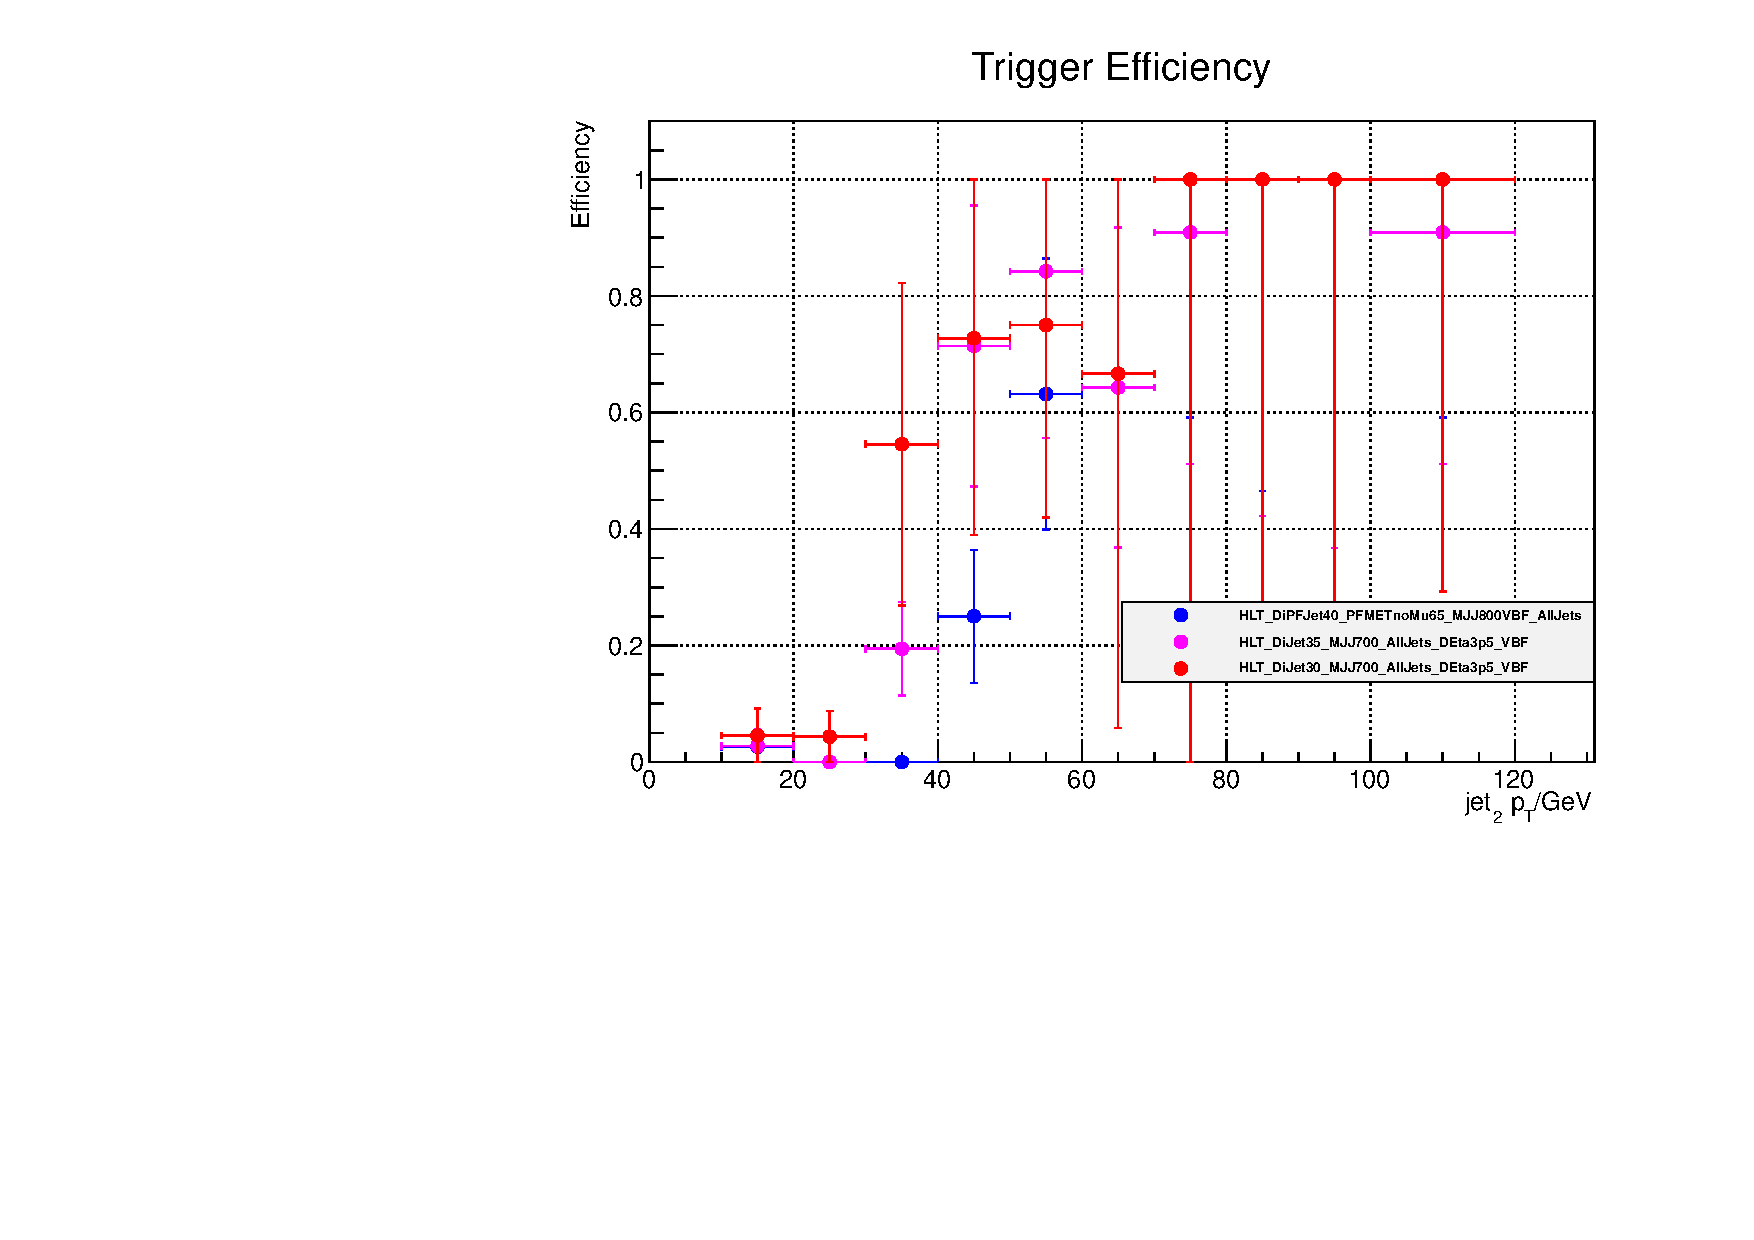
\includegraphics[width=\textwidth]{TalkPics/trigeffplotsallcuts/j2ptefficiency.pdf}
      \end{block}
    \end{columns}
\end{frame}

\begin{frame}
  \frametitle{Conclusions}
  \label{lastframe}

  \begin{block}{}
    \scriptsize
    \begin{itemize}
    \item 1D prompt and parked trigger efficiencies have been measured for Re-Reco data
    \item[-] There are low stats when all cuts are applied so the $\Delta\phi_{jj}$ and CJV cuts have been loosened
    \item 3D trigger efficiency work is in progress
    \end{itemize}
  \end{block}

\end{frame}

\begin{frame}
  \frametitle{Backup}
\end{frame}

\end{fmffile}
\end{document}
